\chapter{Background and Related Work}\label{C:ex}

%%%%%%%%%%%%%%%%%%%%%%%%%%%%%%%%%%%%%%%%
%%%%%%%%%%%%%%%%%%%%%%%%%%%%%%%%%%%%%%%%

\section{Mobile Learning}

Mobile telephony was the operation of mobile phones which enabled users to communicate around freely and wirelessly rather than locate stationary at one fix station. According to \cite{hild1995brief}, the first wireless communication took place in October 23, 1915 when American Telephone \& Telegraph (AT\&T) engineers successfully transmitted radio-telephone signals from Arlington, Virginia to both Paris, France and Pearl Harbour, Hawaii. 

Nevertheless, the first real mobile telephony that used cellular network started much later on, in 1960s, by the Bell Laboratories, USA, when they adopted cellular concept to support hand-held equipment and car telephones. In early 1991, a Global System of Mobile communications (GSM) was introduce as a global protocol of digital cellular network for mobile devices and mobile telephones. Ever since, mobile telephony has gained immense popularity. 

In 1993, less than 10 millions subscribed to mobile service worldwide, by 2003 ten times this number subscribed to the service in China alone \cite{jones2006mobile}. In 2010, nearly half of the world's population was mobile phone owners and this number was forecast to expand to 75 percent in a year period \cite{liu2010understanding}. In 2013, New Zealand Mobile phone owners increased dramatically from 48 percent to 70 percent in 2015 \cite{nzreport}. 

Complemented by the rapid growth of technology, communication not only grew faster, easier and brought people closer together, it also contributed to considerable expansion to education channels. Education platforms have expanded to include mobile-based teaching and learning. According to \cite{mlearningreport} "The worldwide market for Mobile Learning products and services reached \$5.3billion in 2012. The five-year compound annual growth rate (CAGR) is 18.2\% and revenues will more than double to \$12.2 billion by 2017" \cite[pp. 13]{mlearningreport}.

The mobile learning (m-learning) process enabled anywhere any-time learning on mobile devices that supported by communication technology. This section examined the definition of mobile learning and described its potentials and challenges.

%%%%%%%%%%%%%%%%%%%%%%%%%%%%%%%%%%%%%%%

\subsection{Definition of Mobile Learning}

Following the rapid growth of mobile technology and popularity of mobile devices, mobile learning (m-learning) gained more attentions. Much research classified m-learning based on its relationship with electric learning (e-learning). For example, Hoppe et al. (2003) \cite{hoppe2003guest} defined e-learning as the learning that was supported by electronic devices and digital media while m-learning was the delivery of e-learning content via mobile devices and mobile technologies. Similarly, Petrova (2005) \cite{petrova2005mobile} claimed that e-learning and m-learning had the same learning context of physical separation between teachers and learners and the learning process was facilitated by communication technologies, however mobility that enabled learning anywhere any-time differentiated m-learning from e-learning. 

Other research used special characteristics such as "mobility" and "ubiquity" to further differentiate mobile learning (m-learning) from other types of learning. For example, Shudong \& Higgins (2005) \cite{shudong2005limitations} defined m-learning as learning ubiquitously and movably through mobile devices such as mobile phones, Personal Digital assistance (PDA), and iPOD. Lui et al. (2010) \cite{liu2010understanding} agreed that mobile devices and mobile technologies in m-learning allowed people to gain knowledge and skills in ubiquitous manners. Dong (2016) \cite{dong2016mobile} provided a further support that m-learning would contribute as powerful method for ubiquitous learning. 

Focusing on the mobility characteristics of m-learning, Vavoula \& Sharples (2002) \cite{vavoula2002kleos} provided further clarification on its definition that learning could be considered as "mobile" if it was mobile in terms of: location where learning could happen anywhere at workplace or at home; between different aspects in daily life such as learning for self improvement, self entertainment, or as demanded from work; time when learning could happen any-time during the day, on weekdays or weekends. Sharples \& Spikol (2017) \cite{sharples2017mobile} concurred that m-learning had mobility in physical space and was blended into the learners' daily activities and they further added that m-learning also had: 
\begin{itemize} 
\item Mobility of technology - mobile devices were light weight and portable, learners could easily carry these learning resources around, and it allowed them to transfer data between devices
\item Mobility in conceptual space - it allowed learners to explore several learning topics simultaneously as they desired
\item Mobility in social space - it allowed learners to participate within various learning groups such as family, colleagues, and classmates
\item Ability to disperse over time - it had access to cloud storage that cold save knowledge and learning experience, and support accumulative learning. 
\end{itemize} 

Additionally, Pozzi (2007) \cite{pozzi2007impact} refined the definition of mobility by pointing out that learning with devices that were too large to be held comfortably such as laptops, netbooks and some tablets could not be considered as m-learning because of its size and weight. Such learning did not adhere to the anywhere concept of the mobility characteristics. 

Besides, the technological aspect, Berge et al. (2013) \cite{berge2013handbook} included pedagogical, context, and social interaction aspects to defining m-learning. They stated that m-learning was "learning across multiple context, through social and content interactions, using personal electronic devices." \cite[pp. 4]{berge2013handbook}. They further explained that the learning could be either self-directed learning or directed by others; happen either inside or outside a classroom; be a planed or an unplanned spontaneous learning experience. 


On the other hand, O'Malley (2003) \cite{o2003guidelines} argued that m-learning should be defined from a learner's point of view. For instance, m-learning should enable a learner's knowledge acquiring process to happen everywhere, such as a university student viewed class lectures on a bus, doctors read medical journals on their mobile phones en-route to their workplaces, or a language student listened and practised conversations when travelling on a plane. These informal learning activities happened when people were on the move without any use of advanced technologies. Hence, the definition of m-learning was suggested to be widened to "Any sort of learning that happens when the learners is not at fixed, predetermined location, or learning that happens when the learner take advantage of the learning opportunities offered by mobile technologies" \cite[pp.7]{o2003guidelines}. Likewise, Lohnari (2016) \cite{lohnari2016mobile} also defined m-learning on the learner aspect as when learners took advantages of mobile devices to support learning process on their move. 

Based on these perspectives, mobile learning was in essence an extension of e-learning, although differentiated by its mobility and ubiquitous characteristics. It could be defined as the process of teaching and learning across multiple context via mobile devices supported by communication technology to enable learning anywhere when learners were not at a fixed location and any-time. 
	
%%%%%%%%%%%%%%%%%%%%%%%%%%%%%%%%%%%%%%%

\subsection{Potentials of Mobile Learning}

Mobile learning has immense potential to help advance and enhance teaching and learning process. This potential has been widely recognized and highlighted in various researches and initiatives.
The United Nations (UN) developed a set of eight Millennium Development Goals (MDG). One of the goals identified a target towards achieving universal primary education stated "ensure that, by 2015, children everywhere, boys and girls alike, will be able to complete a full course of primary schooling" \cite[pp. 24]{unreport}. In 2015, the UN drew new agenda under this MDG to focus attention on primary schooling for specific groups of children such as those from minorities and communities, children with disabilities, children involved in child labour, and children who lived in urban slums. 

A learner research study by Attewell \& Webster (2005) \cite{attewell2005engaging} was evidential of m-learning's potential to help accomplish this goal. Their study explored learners and mentor's experience towards using smartphones and PDA/phone to seek learning support. They found that m-learning developed learning confidence in a homeless learner who left school and inspired him/her to seek further assistance to improve his/her skills.

Research studies by Fern{\'a}Ndez-L{\'o}Pez et al. (2013) \cite{fernandez2013mobile} and Skiada et al. (2014) \cite{skiada2014easylexia} were the other evidential of the potential. In the \cite{fernandez2013mobile}, Fern{\'a}Ndez-L{\'o}Pez et al. (2013) developed an m-learning application on iOS devices to support students with special education needs aiming to develop their cognitive abilities, help them to learn new knowledge, improve their behavior, communication, and relationship with environment. The application was called "Picca", had four educational activities: exploration, association, puzzle and sorting, and could be personalized by teachers to suite each individual learners. Figure 2.1 presents the four activities design on Ipad and Ipod touch. Picca was used by 39 learners with special education needs from Spain. Observation results showed that the learners' basic skills in language, mathematics, environment awareness, autonomy and social have been improved. 

\begin{figure}[!hbt]\centering
    \begin{subfigure}{0.3\textwidth}
 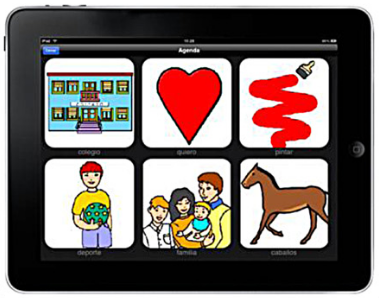
\includegraphics[width=\textwidth]{poten1}
 \caption{Exploration on Ipad}
    \end{subfigure}\hspace{0.1\textwidth}
    \begin{subfigure}{0.3\textwidth}
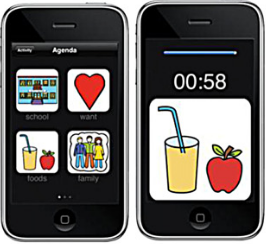
\includegraphics[width=\textwidth]{poten2}
  \caption{Exploring on Ipod}
    \end{subfigure}\hspace{0.2\textwidth}
    \begin{subfigure}{0.19\textwidth}
        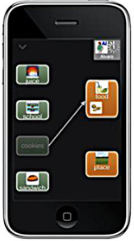
\includegraphics[width=\textwidth]{poten3}
        \caption{Association}
    \end{subfigure}\hspace{0.1\textwidth}
\begin{subfigure}{0.19\textwidth}
        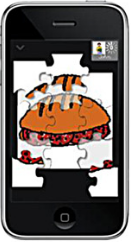
\includegraphics[width=\textwidth]{poten4}
        \caption{Puzzle}
    \end{subfigure}\hspace{0.1\textwidth}
\begin{subfigure}{0.19\textwidth}
        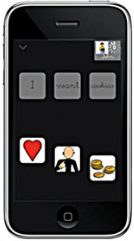
\includegraphics[width=\textwidth]{poten5}
        \caption{Sorting}
    \end{subfigure}
    \caption{Picca's activities \cite{fernandez2013mobile}}
\end{figure}


Similarly, in the \cite{skiada2014easylexia}, Skiada et al. (2014) developed an m-learning application called "EasyLexia" for children with learning difficulties aiming to help the children to improve their reading comprehension, orthographic coding, short-term memory, and mathematical solving. Figure 2.2 presents learning activities provided in EasyLexia application. EasyLexia was used by learners in "Speech Therapy Center", Greece. Even though, the researchers might need more time to assess EasyLexia, their initial observation was promising, indicated that learners made progress in over game performance and had skills improvement. 


\begin{figure}[!hbt]\centering
    \begin{subfigure}{0.25\textwidth}
        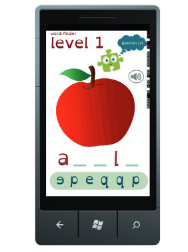
\includegraphics[width=\textwidth]{poten6}
        \caption{Word Finding}
    \end{subfigure}\hspace{0.05\textwidth}
\begin{subfigure}{0.25\textwidth}
        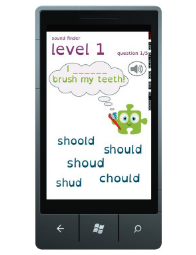
\includegraphics[width=\textwidth]{poten7}
        \caption{Choosing It}
    \end{subfigure}\hspace{0.05\textwidth}
\begin{subfigure}{0.25\textwidth}
        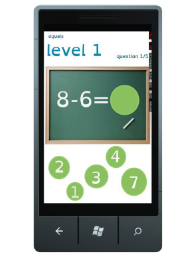
\includegraphics[width=\textwidth]{poten8}
        \caption{Number}
    \end{subfigure}
    \caption{EasyLexia's activities \cite{skiada2014easylexia}}
\end{figure}

Not only could m-learning facilitate education for those specific groups of learners, Klopfer et al. (2002) \cite{klopfer2002environmental} found that running a simulation on PDAs were more cost effective and provided an easier access compared to desktop computer in their land areas investigation. According to them, in the field study, the PDAs offered: 
\begin{itemize}
\item Portability - learners could roam around the areas with the simulation in the PDAs 
\item Social interactivity - learners could share and exchange portable data in their PDAs 
\item Context sensitivity - learners could collect real time data at their current location 
\item Connectivity - learners could easily connect their PDAs to any desktop computer and computer network 
\item Individuality - learners could set their individual observation paths
\end{itemize} 

Traxler (2007) \cite{traxler2007defining} agreed that m-learning had remark potentials to support  authentic learning and provide flexible learning environment when learners approach real work problems in their field study. 

Besides, other research studies discovered m-learning potentials to enhance learning engagement and improve learners' satisfaction. Attewell (2005) \cite{attewell2005research} analysed a large-scale m-learning project across three Europe countries (Italy, UK, and Sweden). In the project, teachers created learning material on desktop computers and learners accessed to the materials from their mobile phones. The adoption of the mobile phones that the learners had been using in their daily lives could encourage computer-resistant learners to learn. In addition, they found the m-learning project that presented the plain, boring, and formal learning content  in attractive and entertainment manners, could engage young learners for a longer period of time. 

Evans (2008) \cite{evans2008effectiveness} and Manuguerra \& Petocz (2011) \cite{manuguerra2011promoting} also found potentials of m-learning to engage and satisfy learners. In the \cite{evans2008effectiveness}, Evans (2008) adopted Podcasting technique that pre-recording learning content into an audio or a video file and learners could download and play the file on their mobile devices to teach first year undergrad learners at University of London, United Kingdom. They found that learners satisfied and preferred Podcasting over attending lectures. 

In the \cite{manuguerra2011promoting}, Manuguerra \& Petocz (2011) observed the adoption of Apple's iPad in both within university setting and distance learning. Within the university, the iPad that was used to present lecture's slides. It, meanwhile, was used to deliver lecture's videos and handle learners' enquiries in the distance learning. The iPad received positive acceptance because it could deliver livelier learning content and it introduced a more comfortable communication platform. 

Ultimately, Corbeil \& Valdes-Corbeil (2007) \cite{corbeil2007you} and Jacob \& Issac (2014) \cite{jacob2014mobile} pointed out potentials of smart phones m-learning to communications and collaborations. Corbeil \& Valdes-Corbeil (2007) \cite{corbeil2007you} claimed that smart phones were more adaptable as an m-learning tool when compared to other hand-held devices owing to its unique combination of communication and computing features in a single device. Jacob \& Issac (2014) \cite{jacob2014mobile} agreed that features on smart phones such as camera, MP3 player, its accessibility to the internet supported collaboration learning and enabled situated learning discussed in other studies. 

In conclusion, the development of mobile devices and communication technology introduced m-learning that brought many potentials supporting specific children learners who could not attend school or had learning difficulties. It enabled flexible access to learning regardless of time and location. Further more, it enabled the delivery of digital media within learning content to help satisfy and engage learners. Ultimately, the smart phones m-learning combined computing and communication technology to support collaboration learning. 

 
%%%%%%%%%%%%%%%%%%%%%%%%%%%%%%%%%%%%%%%

\subsection{Challenges of Mobile Learning}

Notwithstanding immerse potentials, m-learning still had it challenges. Although people own mobile devices with the latest communication technologies, it did not guarantee that they would drop m-learning. Much research recognized this challenge and attempted to find the reasons inhibiting people from adopting m-learning. 

Several years ago, despite a prior report from World Health Organization (WHO) in 2000 \cite{repacholi2001health} that there had no correlation between exposure to mobile phones' radio frequency and adverse health risk, Shudong \& Higgins (2005) \cite{shudong2005limitations} discussed that health concerns might limit the m-learning adoption as many people felt apprehensive towards undesirable health risks associated with mobile usage. 

In later years, there were a difference of opinion regarding to the effect of radio frequency and human health. For example, L{\"o}nn et al. (2004) \cite{lonn2004mobile} found no increased risk of acoustic neuroma associated with short-term mobile phone usage, Thom{\'e}e (2011) \cite{thomee2011mobile} found indirected affects of long-term mobile phone usage to sleep disturbances and depression. Meanwhile, Suhang et al. (2016) \cite{suhag2016impact} who conducted a quantitative study on the impact of mobile phone usage and human physical structure, based on 150 doctors from three different hospital, found that the doctors believed the wireless devices were accountable for the development of diseases of brain tumour, male infertility, and hearing function. Due to the conflicts in existing reports, the health concerns could not be dismissed. It might more or less affected m-learning adoption. 

Furthermore, Shudong \& Higgins (2005) \cite{shudong2005limitations} found that people lacked of psychological motivation to used their mobile devices to learn when they were at home but preferred to do so when they were on their move. The lack of psychological motivation might go along with the lack of appreciation. According to Liaw \& Huang (2012) \cite{liaw2012case}, learners' appreciation towards learning tasks and the perceived long term rewards of acquiring knowledge incentivized users to adopt m-learning. 

On the other hand, Liew et al. (2010) \cite{liaw2010investigating} observed learners' willingness to use a mobile individual knowledge management system implemented on mobile phones. The system provided features to assist learners in managing knowledge they retrieved from online websites. They argued that learners would adopt m-learning system if: the learners perceived m-learning's quality of activities and functionalities; the m-learning system could enhance learner's satisfaction; and the m-learning could promote learners' autonomy. 

Aside from the concerns of negative health impact and the lack of motivation and appreciation towards m-learning, Liu et al. (2010) \cite{liu2010understanding} discussed that the perceived quality of m-learning system and learning content might also affect m-learning adoption. 

In technical perspective, to ensure the portability, the size of mobile devices must be limited. This consequently introduced some hardware limitations such as such as small screens, low resolution, and small keyboard and software limitations such as less features and incompatibility in multiple operating systems that had some negative impacts on the perceived of m-learning quality. There were mixed results found in the observation of the effects of the hardware limitations. 

Firstly, Chae \& Kim (2004) \cite{chae2004size} the screen size was actually had no impact on perception and navigation behavior on mobile internet users in some easy task such as checking e-mail. However, when the task required relatively complex search operations such as buying a gift on a website, the small screen size requited more scrolling and their displays also changed more extensively. These caused difficulties in focusing with the shopping activity. 

To relief this challenge, recent Cascading Style Sheets 3 (CSS3) Media Queries could automatically re-format content on the websites to be appropriately displayed on mobile devices' screen. Alternatively, there were many tools such as Mobify\footnote{\url{https://www.mobify.com/}} and Wirenode\footnote{\url{http://www.wirenode.com/}} that provided some mobile' user interface designs and code blocks that can easily be installed into exiting desktop website. If users used mobile web browser, they would be automatically re-directed to the mobile website version. Figure 2.3 presents browsing some websites in desktop and mobile versions. 
\begin{figure}[!hbt]\centering
    \begin{subfigure}{0.25\textwidth}
 
\includegraphics[width=\textwidth]{cha1}
 \caption{Desktop version}
    \end{subfigure}\hspace{0.1\textwidth}
    \begin{subfigure}{0.25\textwidth}
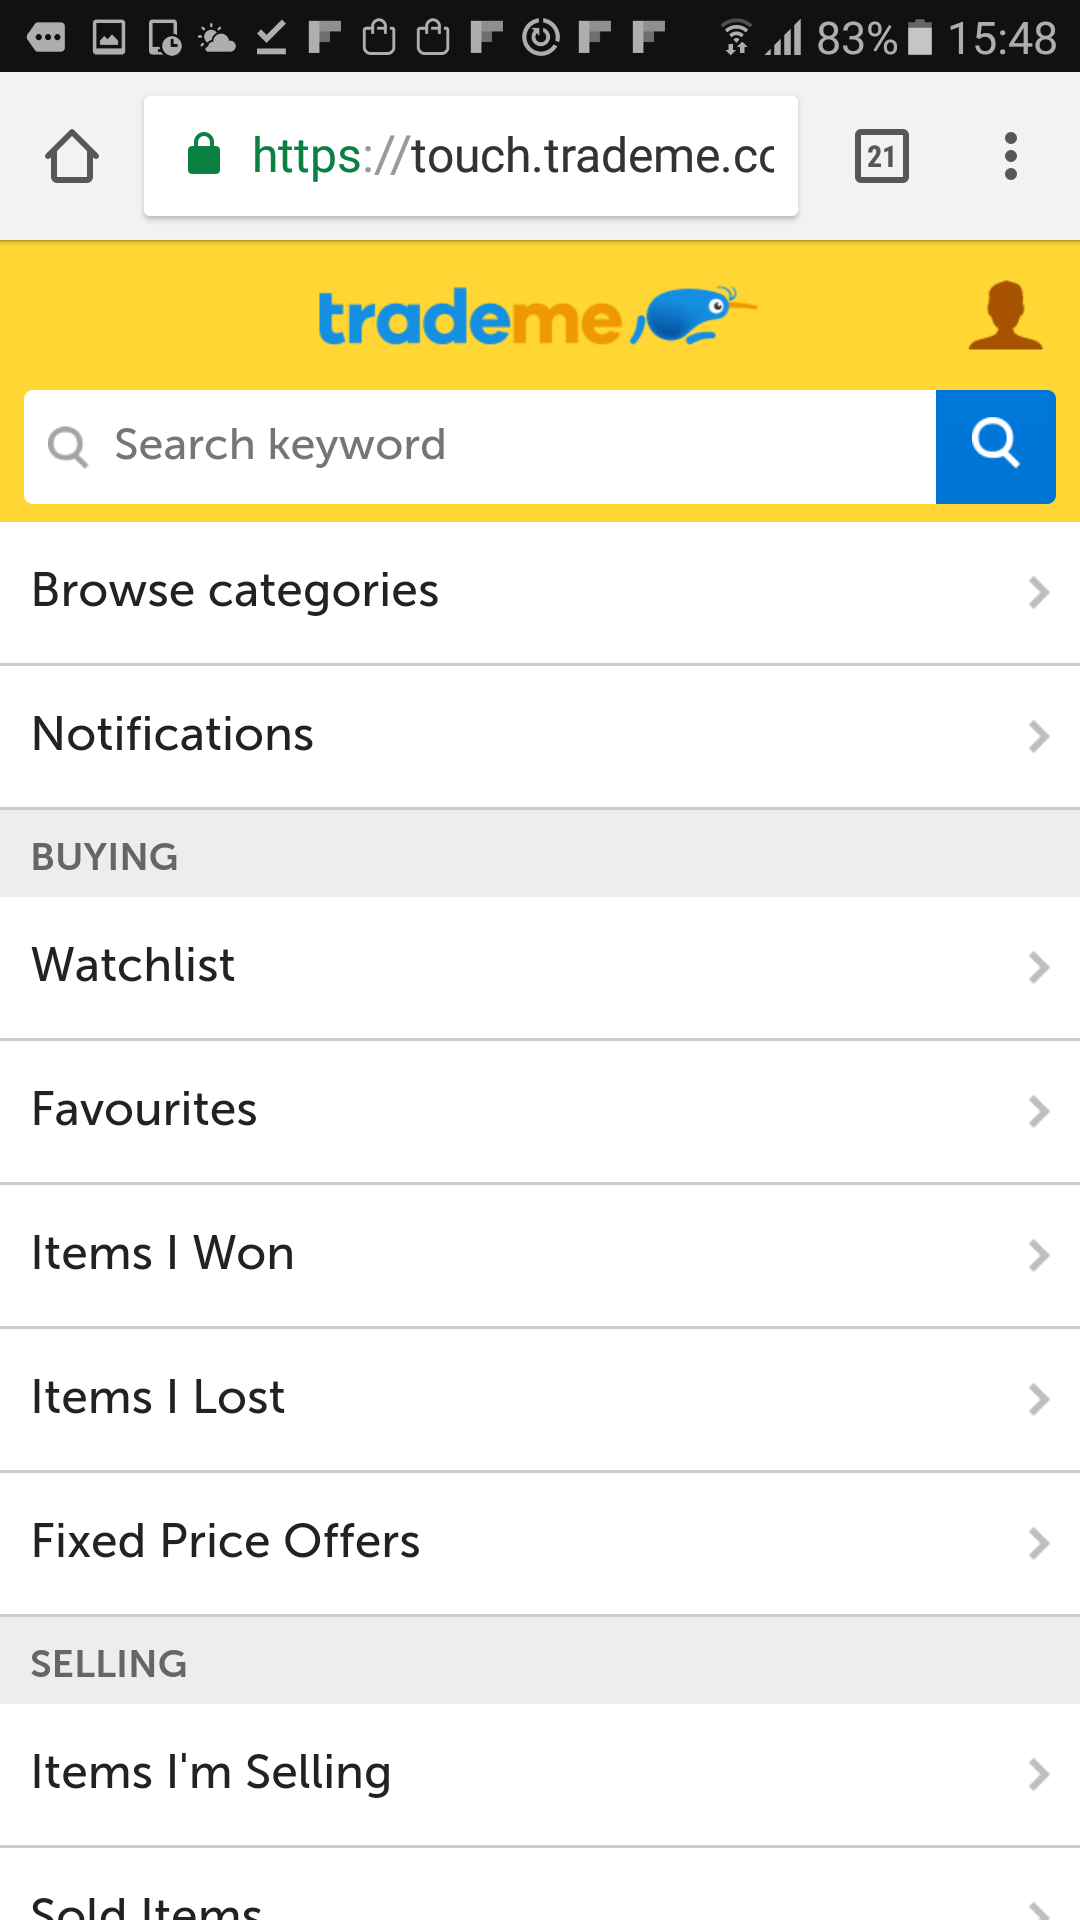
\includegraphics[width=\textwidth]{cha2}
  \caption{Mobile version}
    \end{subfigure}
    \caption{Browsing New Zealand online shopping website "Trademe" in desktop and mobile versions (The screen shots were taken from https://www.trademe.co.nz/ on August, 2017}
\end{figure}

Secondly, Chittaro (2006) \cite{chittaro2006visualizing} pointed out that some visual presentations would also affected by the hardware limitations of the mobile devices. For example pictorial information such as figures, charts, maps, or diagrams that might require a lot interactions such as zooming and scrolling to be viewed on the small screen; rendering 3-dimensional model might suffered from short batter life and lo resolution; and abstract data such as financial trading information posed design challenge for small devices owing to the difficulty in displaying large volume of data against varying time units.

However, these challenges could be diminished by some existing design techniques. For example, Lui et al. (2003) \cite{liu2003automatic} proposed an image attention model that simulated human browsing behavior and automate scrolling large pictures on small screen for users; Chittaro (2006) \cite{chittaro2006visualizing} suggested carry out the rendering of 3-dimensional model on a desktop computer and the results captured and transferred to mobile devices and made available as a video sequence; and the abstract data could be presented in multiple levels of details using fish-eye view. 

Thirdly, Cochrane \& Bateman (2010) \cite{cochrane2010smartphones} observed an implementation of mobile Web 2.0 on smart phone. They found that the choice of smart phones had a critical impact on acceptance of its use. To facilitate social collaboration, smart phones should be able to, for example: capture image and video; stream video; and provide touch screen function, good mobile web experience, and ease of user interface. Furthermore, in language study that learners needed to practice a lot of writing, Godwin-Jones (2011) \cite{godwin2011emerging} found that learners faced difficulties to perform such task on the T9 keyboard of some early mobile phones. However, these observed limitations had become less material to m-learning adoption as the recent rapid growth in communication technology resulted in a much wider range of smart phone choices that are rich in features (Figure 2.4a) and later generation smart phones introduced larger virtual keyboards and touch screens to aid easier text entry (Figure 2.4b).

\begin{figure}[!hbt]\centering
    \begin{subfigure}{1.0\textwidth}
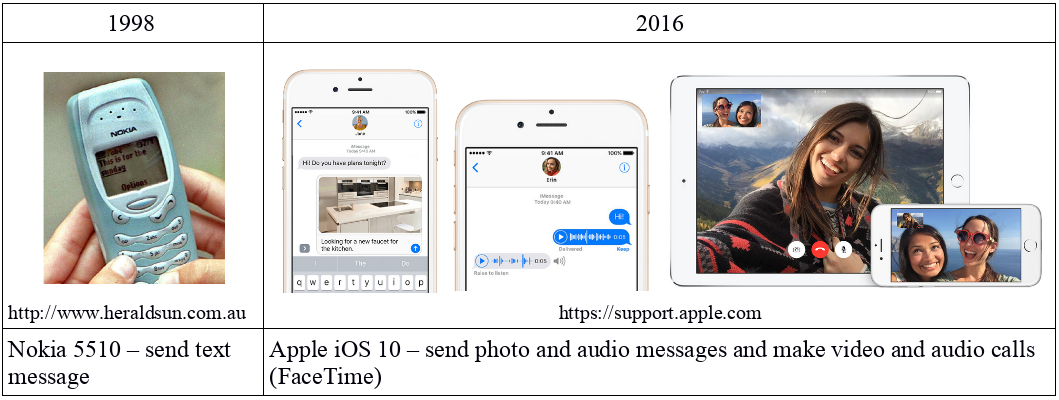
\includegraphics[width=\textwidth]{cha5}
\caption{Early text messaging and recent communication technology}
    \end{subfigure}\hspace{0.1\textwidth}
 \begin{subfigure}{0.55\textwidth}
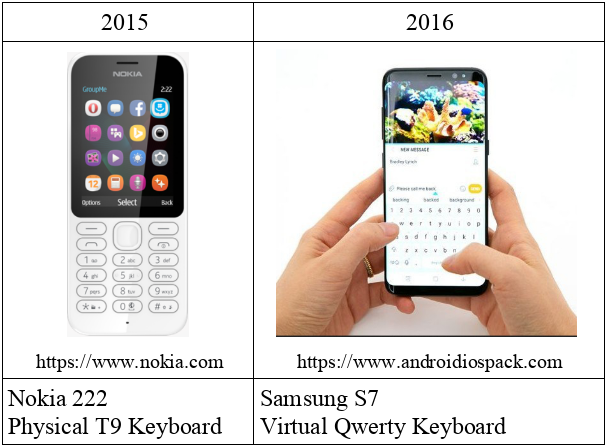
\includegraphics[width=\textwidth]{cha4}
\caption{Physical T9 and virtual qwerty keyboards}
 \end{subfigure}
  \caption{Comparison of early mobile phones and recent smart phones' keyboard and communication features}
\end{figure}

Lastly, Alghamdi et al. (2013) \cite{alghamdi2013impact}  observed of smart phones' screen sizes on patients with normal vision's reading of health information. Samsung Note 10, Note 2, and Galaxy 3 Mini were used to represent large, medium, and small screen size respectively. They argued that the screen size of smart phones did not affected readability, it rather had impact on users' reading concentration and the readability was actually affected by the size of the text. However, neither screen size nor text size had less effects to recent m-learning adoption as later generation smart phones introduced increasingly larger screen sizes (Figure 2.5a) and ability to zoom in and out (Figure 2.5b). 

\begin{figure}[!hbt]\centering
    \begin{subfigure}{0.8\textwidth}
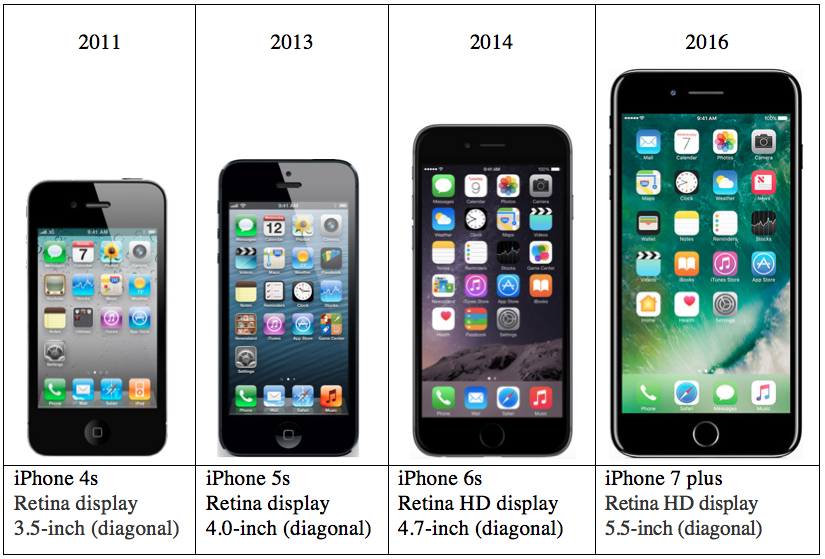
\includegraphics[width=\textwidth]{cha3}
\caption{Revolution of Apple's iPhone}
    \end{subfigure}\hspace{0.1\textwidth}
 \begin{subfigure}{0.8\textwidth}
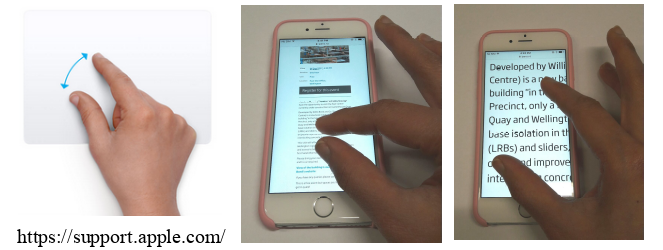
\includegraphics[width=\textwidth]{cha6}
\caption{Apple's two-fingers gestures to zoom in and out}
 \end{subfigure}
  \caption{Apple's iPhone screen size and its ability to zoom with two-fingers gestures for reading small text}
\end{figure}

In pedagogical perspective, m-learning also faced some challenges. Firstly, same with other learning, Shudong \& Higgins (2005) \cite{shudong2005limitations} discussed that m-learning introduced difficulties validating learners' learning progress and achievement. As learning activities could be carried out anywhere and any-time without instructor's supervision, it would be difficult to ascertain any assessment or examination was truly completed by the registered learners themselves.

This pedagogical challenge could be diminished by some advance computer algorithms. For example, Kaiiali et al. (2016) \cite{kaiiali2016designing} proposed a Secure Exam Management System (SEMS) that enabled a secured mobile examination. The system provided m-learning security services such as biometric-based authentication service for anti-impersonation and limit online access during the exam period. They adopted face recognition technology as the biometric-based authentication which was used in conjunction with user name and password pre-authentication. After a learner had successfully processed their login, the system would captured his/her face and would ask the learner to present his/her face to the camera in random basis. Meanwhile, the system control learners' access to some online resources using a Security Agent (SA) that was pre-installed into the learner's device. The SA controlled some access policies such as blocking all Bluetooth, Wi-Fi, and cellular communications accept any connection to an exam server. In order to prevent the learner to manually disable the SA, it periodically sent heart beat to the exam server to ensure its active status (Figure 2.6). 

\begin{figure}[!hbt]\centering
 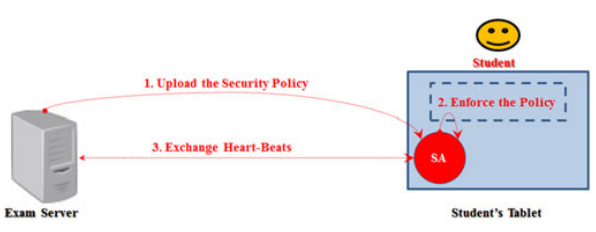
\includegraphics[width=\textwidth]{cha7}
    \caption{Security Agent (SA) strategy \cite{kaiiali2016designing}}
\end{figure}

Secondly, Corbeil \& Valdes-Corbeil (2007) \cite{corbeil2007you} further added m-learning might cause in equality as computer-literate learners could benefit more from the learning process whilst it might trigger isolation for learners who were less proficient in using mobile technologies. The advance of communication technologies such as FaceTime communication (See figure 2.4a) allowed easy communication between the learners and their teachers. The learners could ask questions and the teachers could track the learners' progress, encourage any learners who were falling behind in learning process, and provide individual feedback to them. 

Thirdly, Pozzi (2007) \cite{pozzi2007impact}, Corbeil \& Valdes-Corbeil (2007) \cite{corbeil2007you}, and Cochrane \& Bateman (2010)\cite{cochrane2010smartphones} expressed a concern towards teachers who might need to spend extra efforts to adapt existing teaching material suitable for presentation on smaller screen sizes and additionally prepare the materials in multiple versions to cater to different mobile devices' operating systems. If the teachers were not familiar with mobile technologies, they would require further training at initial stage of the m-learning implementation in order to become accustomed to their roles. 


Throughout the past years, the adoption of m-learning might be inhibited by factors such as concerns with health risks associated with using mobile devices, lack of psychological motivation, hardware and software limitations, and pedagogical challenges. These challenges, however, had been overcome or could be diminished owing to the mobile devices' hardware and software development, advance communication technologies, and expanding knowledge of m-learning implementations. 

The proposed solutions in this section was effectively solve some design challenges for m-learning, it, however did not guarantee learning success. Designing an m-learning course still required an effective design guideline that leaded developers through concrete steps to ensure learning quality.   

According to O'Malley et al. (2003) \cite{o2003guidelines}, design guideline was ``Rules or principles of action, encapsulating some combination of practitioner-determined best practices in a domain and research-based insights into factors relevant in that domain'' \cite[pp. 7]{o2003guidelines}. This, therefore, developing an m-learning design guideline seemed to be problematic because it was a new education platform that had only a little best practice to draw upon. 

Some existing instructional guidelines for actual classroom such as Perkins (2008) \cite{perkins2008smart}'s smart school concept that suggested three characteristics of working together systematically, providing positive energy, and treating each other mindfully also had only little contributions to developing m-learning design guideline  because m-learning rather had individual and independent characteristics. 

Psychological theory, on the other hand, explained reasons behind the individual learners' behavior and enabled developers to predict learning outcomes had more contributions toward developing the m-learning design guideline. Many psychological theories such as Transactional Distance Theory (TDT), Cognitive Load Theory (CLT), Media Richness Theory, Theory of Andragogy, and Activity Theory (AT) were found contributing to design of modern distance education platform such as e-learning and m-learning. 


%%%%%%%%%%%%%%%%%%%%%%%%%%%%%%%%%%%%%%%%
%%%%%%%%%%%%%%%%%%%%%%%%%%%%%%%%%%%%%%%%
\newpage 
\section {Transactional Distance Theory} 

Transactional Distance Theory (TDT) was a theory in distance education that pointed out a special characteristic of physical separation between learners and their teachers. Due to the separation, learners might perceive isolation, encounter communication barriers, and found difficulties to manage their own learning. TDT further identified the elements that caused these issues contributing to a better understanding of such education. This section presents how the theory was developed, defined the elements and explained how they affected quality of distance teaching and learning, and introduces applications of TDT to e-learning and m-learning. 

%%%%%%%%%%%%%%%%%%%%%%%%%%%%%%%%%%%%%%%%%%%%%%

\subsection{Development of Transactional Distance Theory}

Transactional Distance Theory (TDT) was a long-standing  theory. It had celebrated the \nth{40} anniversary in 2013. It had been through the beginning period when the distance education was first recognized, to development period, and ultimately recognized as a value theory in distance education. 

In 1972, Michael G. Moore \cite{moore1972learner} found no systematic theory that explained a non-traditional teaching-learning when learners learnt apart from their teachers. He raised this concern at at the World Conference of the International Council for Correspondence Education (ICCE). Soon after, such teaching and learning was acknowledged as a distance education. This, too, the beginning of TDT. 

The following year, 1973, based on relevant scholars analysis, he defined the distance education as 
\newline 
\newline \textit{"An educational system in which the learner is autonomous, and separated from his teacher by space and time, so that communication is by print, electronic, or other non-human medium"} \cite[pp. 663]{moore1973toward}.
\newline 

Due to the physical separation, learners and teachers might never speak or personally know each other at all, learning material would be used upon learners' decision outside the teachers' control, and the learners needed to take control of their own learning process. Based on this natures of distance education, Moore (1973) \cite{moore1973toward}, also discovered three elements: dialogue, course structure, and learner autonomy that affected distance education.

In the next decade, 1983, Moore \cite{moore1983individual} introduced "transactional distance" to come after the psychological perception of physical separation in distance education. He claimed that the transactional distance was a special characteristic of such education. Even though, learners in traditional classroom might separate with their teachers at some stage, the transactional distance within this educational setting was narrow because the learners had chances to have some verbal communications with their teachers. On the other hand, the transaction distance within distance education was wider because learners and teachers would only communicate through printed or electronic media. 

Besides the emerging of the transactional distance, the definitions of dialogue, structure and learner autonomy also became explicit. Moore (1983) \cite{moore1983individual} defined: 
\newline 
\newline \textit{The dialogue - two-way communication between learners and teachers}
\newline 
\newline \textit{The structure - an educational program's responsiveness to identify learning objectives, implement learning program, and evaluate learning outcomes to meet learners' individual needs}
\newline 
\newline \textit{The autonomous learner - a learner who could identify required skilled and information that helped them to approach their learning problems, able to set their own learning goals and achievement criteria, effectively carry out their own learning process, and able to value their learning experience and knowledge.} 
\newline 
\newline Additionally, Moore (1980; 1983) \cite{moore1980independent, moore1983individual} proposed four types of distance education programs that were generated from the interplay of dialogue (D) and structure (S). Figure 2.xa - 2.xd illustrates the teaching-learning relationship of the four types of distance education programs. "A" represented a teacher while "B", "C", "D", and "E" represented learners. 

\begin{figure}[!hbt]\centering
    \begin{subfigure}{0.3\textwidth}
 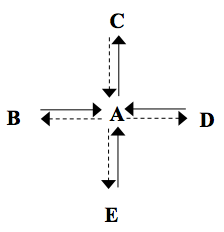
\includegraphics[width=\textwidth]{tdt1a}
 \caption{-D-S}
    \end{subfigure}\hspace{0.15\textwidth}
    \begin{subfigure}{0.285\textwidth}
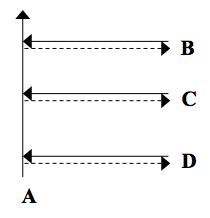
\includegraphics[width=\textwidth]{tdt1b}
  \caption{-D+S}
    \end{subfigure}
    \begin{subfigure}{0.285\textwidth}
        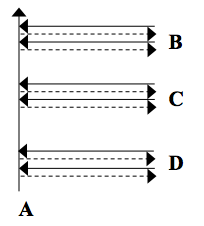
\includegraphics[width=\textwidth]{tdt1c}
        \caption{+D+S}
    \end{subfigure}\hspace{0.15\textwidth}
\begin{subfigure}{0.36\textwidth}
        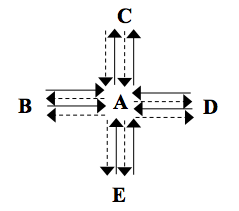
\includegraphics[width=\textwidth]{tdt1d}
        \caption{+D-S}
    \end{subfigure}
    \caption{Teaching-learning relationship of distance education programs \cite{moore1983individual}}
\end{figure}

\begin{itemize}
\item \textbf{-D-S} represented a program with no dialogue and no structure (i.e., flexible and one-way communication programme) such as self-directed study
\item \textbf{-D+S} represented a program with no dialogue but with structure (i.e., high structural and one-way communication programme)  such as radio and television 
\item \textbf{+D+S} represented a program with dialogue and structure (i.e., high structural and two-way communication programme) such as correspondence programme  
\item \textbf{+D-S} represented a program with dialogue and structure (i.e., flexible and two-way communication programme) such as tutorial program 
\end{itemize}

 
The distance were qualitative, the -D-S caused the most distance because it was a self-study that learners needed to plan, implement, and evaluate their own learning. On the other hand, the +D-S had the lest distance because it allowed the learners to communicate with teachers. However, this type of distance course did not allow learners to exercise much of their autonomy because the teachers might lead most of the teaching-learning processes. 


Besides D and S, Moore (1980; 1983) \cite{moore1980independent, moore1983individual} also employed learner autonomy to classified distance education. He identified if three activities: goal setting, implementation, and evaluation had been done by learners or teachers. The "A" represented autonomous which referred to learners determined the process while "N" represented non-autonomous which referred to teachers determined the process. Table 1 presents type of distance learning programs classified by learner autonomy. 

\begin{table}[!htb]
\centering
\caption{Type of distance learning programs classified by autonomy \cite{moore1980independent}}
\begin{tabular}{ |c|c|c| } 
 \hline
 Goal Setting & Implementation & Evaluation \\ 
\hline
 A & A & A \\ 
\hline
 A & A & N \\ 
 \hline
 A & N & A \\ 
\hline
 A & N & N \\ 
 \hline
 N & A & A \\ 
\hline
  N & N & A \\ 
 \hline
  N & A & N \\ 
\hline
  N & N & N \\ 
 \hline
\end{tabular}
\end{table}

The classification ranged from those programme that allowed learner to maximum control over all three process (AAA) to those programme that allowed only a little autonomy (NNN). The most common type of learning would probably NAN that learners took control over their learning processes, however, the teachers set learning objectives and they took control over the evaluation process. The lest common type of learning were NAA and NNA because it was rarely that teachers set learning goals but allowed learners to evaluate themselves. 

\newpage
This Learner autonomy classification could be plotted in three-dimension diagram (Figure 2.x), too, placed against distance in two-dimension diagram (Figure 2.x)
\begin{figure}[!hbt]
\centering
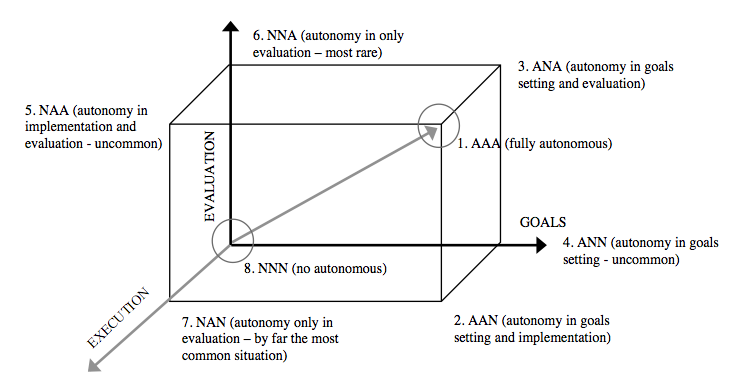
\includegraphics[width=1.1\textwidth]{tdt2}
\caption {Three-dimension autonomy classification of distance program \cite[pp. 73]{moore2013handbook}}
\end{figure}

\begin{figure}[!hbt]
\centering
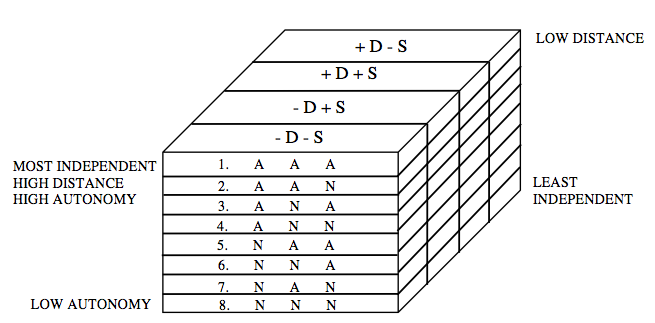
\includegraphics[width=0.85 \textwidth]{tdt3}
\caption {Typology of educational program classification \cite[pp. 73]{moore1983individual}}
\end{figure}

In the next decade, 1993, Moore \cite{moore1993theory} formed Transactional Distance Theory (TDT) to explain the special characteristic of separation of teachers and learners in distance education. Figure 2.x summarized the development of TDT. 

Due to the physical separation, both parties might never meet or hardly have any conversation, the learners needed to take control over their own learning, and potentially perceive transactional distance that decrease learning quality. There were three elements that varied the transactional distance: dialogue between teachers and learners, course structure, and learner autonomy. 

%%%%%%%%%%%%%%%%%%%%%%%%%%%%%%%%%%%%%%%%%%%%%%
\newpage 
\subsection {Dialogue} 

According to Moore (2013) \cite{moore2013handbook}, dialogue was a subset of interaction including words and actions that had positive qualities, purposeful, and constructive. The amount and quality of dialogue were controlled by three factors: philosophy of the course, personality of teachers and learners, learning environment including number of learners, language, and communication media. For example, a single learner was found having more dialogue with teachers compare to a group study of many learners; a learner who shared a same native language with teachers found having more dialogue than learners who used foreign languages; and the course tough through video conference that provide a prompt response found having more dialogue than the the course tough through a mail that provided a slow dialogue. Nevertheless, 


The computer-mediated conference, nevertheless, might not suit some learners. For example in a foreign language course learners found to be rather comfortable with text-based asynchronous communication than direct verbal communication. Even though, the video-conferencing media provided the fasted dialogue, an electronic mail communication would be a better communication choice \cite{moore2011distance}. 

%%%%%%%%%%%%%%%%%%%%%%%%%%%%%%%%%%%%%%%%%%%%%%

\subsection {Course Structure} 

Structure was the structural plan of the course that informed how learning content would be delivered through those communication media. Similar to the dialogue, course structure was a qualitative and dependent variable.

The combination of the media and course structure could determine the quality of teaching and learning \cite{moore1993theory}. Practically, delivering teaching processes through numerous media was a recommended practice, for example, presenting learning content through video recording, evaluating learners' knowledge using correspondence, and providing feedbacks through video conference \cite{moore1993theory}. There had no certain structure for the distance education. Moore (1993) \cite{moore1993theory} suggested launching a pilot-study to observe if learners comfortable with either a high-structured or flexible course. 

In the high-structured course, learners might be instructed to learned as a planned schedule, they could not explore other part of learning without permission, media such as audio or video could be used when allowed, and they could communicate with their teachers within pre-determined time table \cite{moore2011distance}. 

The flexible course structure, on the other hand, gave them opportunities to learn in their desired speed, submit the assignment when they are ready, explore all course materials, and provided communication channel such as electronic mail or help desk that allowed them to contact teachers when needed \cite{moore2011distance}.

Within the structure elements, besides highlighting on the types of media and flexibility of the course structure, Moore (1993) \cite{moore1993theory} suggested six-instructional processes for distance education design: 

\begin{enumerate}
\item Presentation - use either text, audio, or video to present learning content and choose a computer media over a printed media if the content required a frequent update

\item Motivation - use film, text, feedback, or personal dialogues to motivate learners to learn and maintain their interest

\item Stimulation of Analysis and Criticism - arrange discussion sessions with experts for learners or teachers or allow them to hear pre-recorded of the experts' discussion. These processes would help the learners to develop their cognitive skills

\item Advice and Consolation - either within learning materials or through a personal contact such as e-mail, provide some instructions how to use learning materials; suggestions on learning techniques; and references to external learning resources 

\item Practice and Evaluation - allow learners to practice what they had learnt such as providing a writing assignment, evaluate, value their performance especially if they applied some new knowledge, and provide some feedback through an e-mail or discussing session 

\item Creation of Knowledge - allow learners to discuss and share their ideas with teachers though video-conferencing, e-mail, or text. 
\end{enumerate}

%%%%%%%%%%%%%%%%%%% Relationship %%%%%%%%%%%%%%%%

\subsubsection{Relationships between Dialogue, Structure, and Transactional Distance} 

Moore 2013 \cite{moore2013handbook} claimed that ``transactional distance is a function of dialogue and structure'' \cite[pp. 71]{moore2013handbook}. 
\begin{itemize}
\item The course that had high degree of structure and allowed little to no dialogue had high transactional distance
\item That had flexible structure and allowed dialogue through an appropriate medium had less transactional distance
\end{itemize}
The relation between dialogue, structure, and transactional distance could be presented in two-dimension graph (See figure 2.10). 

\begin{figure}[!hbt]
\centering
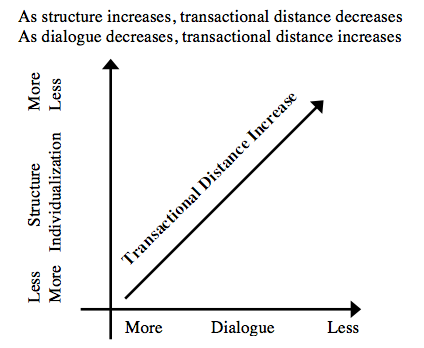
\includegraphics[width=0.65 \textwidth]{tdt4}
\caption {Two dimension of relation between transactional distance and dialogue and structure \cite[pp. 71]{moore2013handbook}}
\end{figure}

%%%%%%%%%%%%%%%%%%%%%%%%%%%%%%%%%%%%%%%%%%%%%%

\subsection {Learner Autonomy} 
Learner autonomy was learners' ability to determine learning goals and make decision on learning process. The learners would use what teachers provided to achieve the goals on their own ways and under their own control \cite{moore1993theory}. The relationship between the learner autonomy and transactional distance were the greater transactional distance the more responsibilities learners had to exercise (See figure 2.11). 

\begin{figure}[!hbt]
\centering
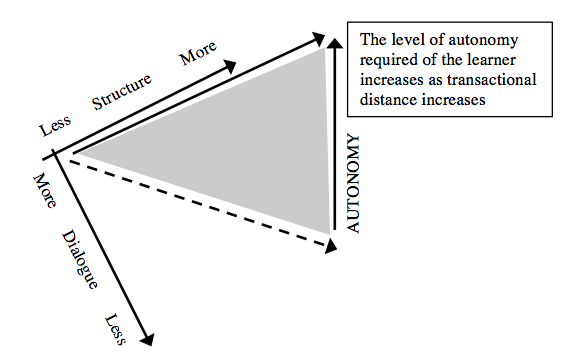
\includegraphics[width=0.65 \textwidth]{tdt5}
\caption {Relationship between transactional distance and learner autonomy \cite{moore1993theory}}
\end{figure}

Based on an empirical study \cite{moore1993theory}, there were patterns of personality characteristics of the learners, dialogue, and course structure - autonomous learners seemed to be comfortable with less dialogue and less structural programme. That is to say, they did not need to communicate with the teachers much and preferred a flexible course structure. Mean while, non-autonomous learners seemed to prefer a programme with more dialogue and much structural programme. 

%%%%%%%%%%%%%%%%%%%%%%%%%%%%%%%%%%%%%%%%%%%%%%
\subsection{Applications of Transactional Distance Theory} 
Since TDT was introduced in 1993, it had contributed to understanding of distance education. Much research adopted the theory as a heuristic tool to observe modern education such as e-learning and m-learning. Other research also proposed transactional distant measurement tool as indications of distance courses' teaching-learning quality. These suggested what aspects of the distance course design needed improvements and ensured the its quality. Despite these contributions, much research argued that TDT did not include a social-cultural aspect and other research criticized that the definition of transactional distance and other elements was not clear enough. This, therefore, leaded to disagreement and conflicts within following studies. 

Benson et al. (2009) \cite{benson2009addressing} adopted TDT as a heuristic tool to to observe the six e-learning courses offered at two Australia universities. They firstly, divided the courses into either low, medium, or high transactional distance (TD). After that, they analyzed how much dialogue the courses provided (D), how the courses were constructed (S), and autonomy of learners (A). Table 2.x presents some examples of their e-learning courses' analysis 

\begin{table}[!htb]
\centering
\caption{Example of distance courses analysis \cite{benson2009addressing}}
\begin{tabular}{ |p{2.5cm}|p{7.35 cm}|p{2.2cm}|} 
 \hline
 Distance Course & Explanation & Analysis\\
\hline
 On-campus and classroom-enhanced course & 1. Low transactional distance course
\newline2. No dialogue in e-learning platform
\newline3. Offered unstructured online material
\newline 4. Autonomous learners however it was not taken into account because it was controlled by teachers & (-D -S +A) \\ 
\hline
Off-campus and partially online course& 1. High transactional distance course
\newline2. Provided dialogue through online discussion in arranged time frames
\newline3. Offered printed materials, DVD of case studies, online learning on the course website, and arranged online discussion sessions
\newline4. Autonomous learners & (+D +S +A)\\ 
 \hline
Workplace-based and blended learning & 1. High transactional distance course
\newline2. Medium transactional distance
\newline3. Dialogue and structure were found to be conversely
\newline4. Unknown learner autonomy  & (+D -S --) or (-D +S --) \\ \hline 
\end{tabular}
\end{table}

Based on the distance course analysis, the study \cite{benson2009addressing} concluded that
\begin{itemize}
\item The low transactional distance e-learning course should disregard learner autonomy and could provide no dialogue and flexible course structure
\item The high transactional e-learning course should disregard learner autonomy and provide dialogue and well-structured course
\item The medium transactional e-learning course, with regards to learner autonomy, should provide converse of dialogue and course structure 
\end{itemize} 

Despite the potential to guide the design of the distance education, Kang \& Gyorke (2008) \cite{kang2008rethinking} pointed out that the theory lacked a social-cultural aspect which was critical in today's practice. They further compared TDT with the cultural-historical theory of activity (CHAT) and stated that "CHAT's tool-mediated and sign-mediated nature of all aspects of human interaction makes more sense with regard to the concept of social learning interaction" \cite[pp.211]{kang2008rethinking} meanwhile "TDT isolates learners from their multi-society context" \cite[pp.212]{kang2008rethinking}. 

With regards to the social aspect, Benson et al. (2009)'s study \cite{benson2009addressing} lacked of consideration of dialogue between learners themselves. This might affected the level of transactional distance. For example, in the off-campus and partially online course which was claimed to have high transactional distance, even though the learners could not contact their teachers, they might contact each other through an e-mail, and this might decrease their perception of transactional distance. 

Similar to \cite{benson2009addressing}, Park (2011)  \cite{park2011pedagogical} adopted TDT to classify available m-learning courses. They, however, realized that mobile technologies allowed learners to communicate not only with their teachers but also among themselves and TDT did not cover this social interaction. Therefore, in order to complete the classification criteria, they added activity theory (AT) as another classification dimension. 

Grounding on TDT, an m-learning course would be classified as high transactional distance if learners perceived psychological and communication barrier with their instructor or teaching and learning activities and materials were predetermined and low transactional distance if they perceived less of those feelings and the course structure was flexible. 

Meanwhile, grounding on AT, an m-learning course would be classified as individualized type if learners could communicate directly to their teachers and their teachers control learning processes and allowed them to maintain their independence. For the socialized type, learners would work together as a group and engaged into social collaboration. 

Based on the classification criteria the studies classified m-leaning into four types and suggested how developers should design m-learning course for each type. Table 2.x presents the m-learning classification grounded on on TDT and AT and its design recommendations. 
\begin{table}[!htb]
\centering
\caption{M-learning classification grounded on TDT and AT and design recommendations \cite{park2011pedagogical}}
\begin{tabular}{ |p{4.5cm}|p{8.5cm}|} 
 \hline
Classification & Design recommendations\\
\hline
Type 1 - High Transactional Distance and Socialized Mobile Learning Activity (HI) & The interface design should encourage social participation. Software and hardware of all devices involved in the m-learning activity should be compatible with each other\\
\hline 
Type 2 - High Transactional Distance and Individualized Mobile Learning Activity (HS) & The learning material such as lecture audio and video should be well-organized. Developers should ensure that individual learners could access to the material remotely\\
\hline Type 3 - Low Transactional Distance and Socialized Mobile Learning Activity (LS) & The m-learning should promote active participation and provided many social collaboration learning tasks such as online discussion, debating, and competition \\
\hline Type 4 - Low Transactional Distance and Individualized Mobile Learning Activity (LI) & Teachers should prepare learning supports when learners had questions and perform their assignments with regards to learning environment either in a classroom or field trip\\
\hline
\end{tabular}
\end{table}

Not only being used as a heuristic tool to observe e-learning and m-learning, Zhang (2003) \cite{zhang2003transactional} proposed a transactional distance measurement survey for a web-based learning environment. In the study transactional distance was "cognitive, emotional, social, cultural, and/or physical distance between learners and other elements of their learning environments that prohibit active student engagement with learning" \cite[pp.148]{zhang2003transactional}. They \cite{zhang2003transactional} hypothesized that transactional distance between student and student, student and teacher, student and learning content, student and web-based interface design might prohibit students to engage with learning. 

The measurement items went through confirmatory factor analyses and exploratory analyses to ensure validity. It had been proven statistically reliable to measure the transactional distance in web-based program. 

Similarly, Wengrowicz et al. (2014) \cite{wengrowicz2014transactional} also developed a transactional distance measurement tool. Their application, however, limited to the transactional distance between peer students in a collaboration and visualization-rich environment. 

Noticeably, these TDT applications (i.e., \cite{benson2009addressing, park2011pedagogical, zhang2003transactional, wengrowicz2014transactional}) interpreted the term transactional distance slightly different. For example, Benson (2009) \cite{benson2009addressing} and Park (2011) \cite{park2011pedagogical}' studies inherited TDT original proposition that the transactional distance increased when dialogue between learners and teachers decreased. On the other hand, Zhang (2003) \cite{zhang2003transactional}' study included relationship between learners and other learners, learning content, and even interface design as the factors that influenced transactional distance. 

Gorsky \& Caspi (2005) \cite{gorsky2005critical} raised the concerns towards different interpretation of the transactional distance given in TDT. They investigated published empirical studies including \cite{saba1994verifying, bunker1996study, bischoff1996transactional, chen2001transactional, chen2001dimensions, chen2007path} that applied TDT in their research. Gorsky \& Caspi (2005) \cite{gorsky2005critical} found that these researchers constructed their empirical studies based on their personal interpretation of TDT of which different from the original proposition. For example, Chen \& Willis (2007) \cite{chen2007path}' study measured frequency of communication as dialogue. This, however, conflicted with original definition of dialogue given in TDT that defined the dialogue as learner understanding. 

Despite the lack in incorporating of social-cultural aspect and ambiguous definition given in TDT, the theory pointed out the existence of transactional distance within distance education and introduced three elements that affected the transactional distance which could be used as a heuristic guide for distance education design to ensure learning effectiveness. 

\section{Other Learning Theories} 

Most of educational design guidelines were grounded on psychological theory because, according to Fosnot \& Perry (1996) \cite{fosnot1996constructivism} it explained about learning which contributed instructional-decision making. 

%%%%%%%%%%%%%%%%%%%%%%%%%%%%%%%%%%%%%%%%%%%%%%%%%%%%%%%%%%
%%%%%%%%%%%%%%%%%%%%%%%%%%%%%%%%%%%%%%%%%%%%%%%%%%%%%%%%%%
\iffalse
\subsubsection {Theory of Learning}
Fosnot \& Perry (1996) \cite{fosnot1996constructivism} introduced three types of psychological theory of learning: behaviourism, maturationism, and constructivism. 

The behaviourism assumed behavior was produced by a response to certain stimuli or consequence of reinforcement, practice, and external motivation. This type of theory, therefore, had less contribution to m-learning because the learning took place in distance and learners learnt autonomously. It was hard for teachers or institution to manage learning environment and reinforce learners. 

The maturationism believed biological factors had more influences to children's learning compared to environment factors. This type of theory also had less contribution to m-learning because it had limited applicability to early childhood education (e.g., Hughes (2016) \cite{hughes2016kindergarten}'s study that applied the theory to explained relationship between kindergarten entry age and the effect on student academic achievement). Meanwhile, most m-learning learners were adults learners who owned a mobile device, knew mobile technologies, and could learn autonomously. 

On the other hand, the constructivism believed that learners constructed their understanding and new knowledge by experiencing things and reflecting on the experiences, seemed to have the most contribution to m-learning because in autonomous m-learning, the learners could roam around and experienced situated learning in field study. 
\fi 

%%%%%%%%%%%%%%%%%%%%%%%%%%%%%%%%%%%%%%%%%%%%%%%%%%%%%%%%%%
\subsection{Cognitive Load Theory} 

In 1998, Sweller et al. (1998) \cite{sweller1998cognitive} introduced Cognitive Load Theory (CLT) which "...has been designed to provide guidelines intended to assist in the presentation of information in a manner that encourages learner activities that optimize intellectual performance" \cite[pp. 251]{sweller1998cognitive}. According to them there were three type of cognitive load: 
\begin{itemize}
\item Intrinsic cognitive load that deals with complexity inherited in learning tasks 
\item Extraneous cognitive load that deals with non-relevant elements such as decorating pictures and animation that required extra mental processing and did not promote learning 
\item Germane cognitive load that actual benefits learning and deals with information processing resulting in schema construction and automation 
\end{itemize}

The three additive cognitive loads was a working memory load that learners need to invest in their learning process. Grounding on the CLT, many studies proposed some instructional design that decreased the working memory load. 

For example, Clarke (2005) \cite{clarke2005impact} claimed that presenting learning tasks with a progressive method (i.e., presenting a simple task first and add more complexity to the task later) would decrease intrinsic cognitive load. In their experiment, they used spreadsheets to assist mathematics learning. One group was trained to use spreadsheet first and learnt about mathematics skills  later (i.e., sequencing learning method). Meanwhile, the other group learnt both skills concurrently. They found that, learners who had no prior knowledge on spreadsheet performed better in the sequent learning compared to the concurrent learning method, however, for learners who had prior knowledge on spreadsheet, the results came out vice versa. Based on these outcomes, sequencing learning tasks from simple of complex had implications to cognitive load, this however was applicable to only learners who had low level of prior knowledge. 

Another example, Schnotz \& Rasch (2005) \cite{schnotz2005enabling} used animation to increase learners' motivation and germane cognitive load. They claimed that, comparing to static image, the animation had enabling function that allowed more interaction and facilitating function that helped learners to understand learning content and eased their cognitive process. These functions could potentially reduced cognitive load. However, unfortunately, they found that using animation did not improve overall learning performance in learners who had low prior knowledge because the facilitating function of animation reduced their germane cognitive load. They, therefore, suggested that animation was only beneficial in some circumstances and might have negative effects in other circumstances. 

%%%%%%%%%%%%%%%%%%%%%%%%%%%%%%%%%%%%%%%%%%%%%%%%%%%%
\subsection{Self Determination Theory}

In distance learning context, learners mostly learnt autonomously and without motivation they might not initiate learning. According to Ryan \& Deci (2000) \cite{ryan2000intrinsic}, "To be motivated means to be moved to do something. A person who feels no impetus or inspiration to act is thus characterized as unmotivated, whereas someone who is energized or activated toward an end is considered motivated.'' \cite [pp. 54] {ryan2000intrinsic}. Deci \& Ryan (1985) introduced Self Determination Theory which was a theory of motivation. They explained that there were two types of motivation: intrinsic and extrinsic motivation. 

The intrinsic motivation, according to Ryan \& Deci (2000), was "the doing of an activity for its inherent satisfactions rather than for some separable consequence.'' \cite [pp. 56] {ryan2000intrinsic}. Malone \& Lepper (1987) further explained \cite{malone1987making} relationship between learning and intrinsic motivations that the intrinsic motivation could be triggered by providing learners with challenge, curiosity, control, fantasy, cooperation, competition, and recognition. 

Schwabe \& G{\"o}th (2005) \cite{schwabe2005mobile} designed a MobileGame prototype grounding on the relationship between learning and intrinsic motivations. It a rally game that used in orientation day that aimed to introduce university surroundings to learners. It displayed position of learners on digital map of hand-held devices. The learners would be asked to perform activities such as answering questions before moving to the other spots. Based on their results, the game had potential to enhance learning, most of the participants enjoyed playing the game, and would like to play it again. 

The extrinsic motivation, according to Ryan \& Deci (2000), was "a construct that pertains whenever an activity is done in order to attain some separable outcome.'' \cite [pp. 60] {ryan2000intrinsic}. This, therefore, contrasted with the intrinsic motivation as learners were motivated by some external rewarding such as good grades and scholarships rather than their personal rewarding. 


Muntean (2011) \cite{muntean2011raising} claimed that both motivations could be co-operated within gamification to raise engagement in e-learning. According to them, the gamification was "the use of game play elements for non-game applications, particularly consumer-oriented web and mobile sites, in order to encourage people to adopt the applications.'' \cite [pp.325]{muntean2011raising}. The gamification intrinsic motivated learners by triggering their sense of competition and cooperation  and extrinsic motivated them with rewards such as level progression, points, and badges. They claimed that the gamification could improve learning performance. 

Nevertheless, Rosenfield (1980) \cite{rosenfield1980rewards} expressed a concern that using rewarding to extrinsic motivated learners might unintentionally decreased their intrinsic motivation which was called "overjustification effects". Therefore, they suggested that if learners had already found that the learning was intrinsically rewarding, the extrinsically rewarding should not be applied. 

%%%%%%%%%%%%%%%%%%%%%%%%%%%%%%%%%%%%%%%%%%%%%%%%%%%%%%
\subsubsection{Long Life Learning} 

The motivation and lifelong learning were closely related, as, according to McCombs (1991) \cite{mccombs1991motivation},"the motivated person is a lifelong learner, and the lifelong learner is a motivated person'' \cite [pp. 117]{mccombs1991motivation}. Same with the motivation, the lifelong learning was a human nature and self-motivated to learn, grow, and develop due to personal curiosity, enjoyment, satisfaction, or professional development. McCombs (1991) \cite{mccombs1991motivation}claimed that the lifelong learning was crucial quality in \nth{21} century education and further suggested how to instructional design a long life learning: 
\begin{itemize} 
\item Structuring the course based on psychological knowledge 
\item Including instructional strategies that motivated learners 
\item Providing adaptive learning context 
\item Providing opportunities to approach real life problem 
\end{itemize} 

Sharples (2000) \cite{sharples2000design} further pointed out that hand-held computer had potential to facilitated a situated learning throughout a lifetime. In order to observe the potential of the tool, they developed a hand-held learning resource (HandLeR). Figure 2.x presents HandLer Interface design of a rabbit mentor (figure 2.2a). Each part of the rabbit's body were the main tools, for example, if learners clicked on the rabbit's brain, it displayed a linked concept (figure 2.2b). 

\begin{figure}[!hbt]\centering
\begin{subfigure}{0.4\textwidth}
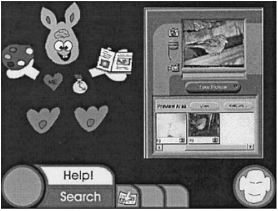
\includegraphics[width=\textwidth]{lifelong1}
\caption{The rabbit mentor}
\end{subfigure}\hspace{0.05\textwidth}
\begin{subfigure}{0.4\textwidth}
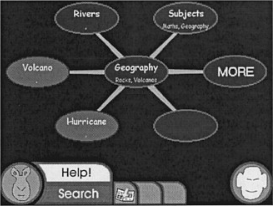
\includegraphics[width=\textwidth]{lifelong2}
\caption{The rabbit's brain tool}
\end{subfigure}
\begin{subfigure}{0.35\textwidth}
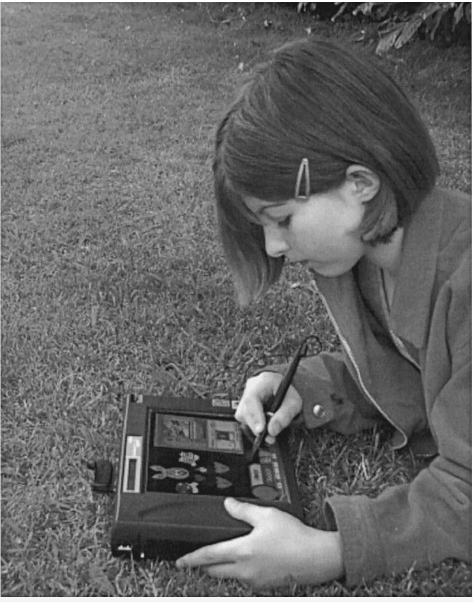
\includegraphics[width= \textwidth]{lifelong3}
\caption{HandLer in use}
\end{subfigure}
\caption{HandLer interface design \cite{sharples2000design}}
\end{figure}

Based on their observation, they analyzed the tool' software, hardware, communications, and interface design requirements. To be able to appropriately support a lifelong learning: 
\begin{itemize}
\item Software should be able to store; organized and retrieve events; structure and process knowledge for a long period of time; and handle adaptive learning context
\item Hardware should be highly portable; adaptable to individual's abilities, skills, and knowledge, unobtrusive; available for communication anywhere; persistent to manage learning for a long period of time; useful in daily activities; and intuitive to be used by technology novices
\item Communication should be able to alter its bandwidth to match learners' demand and automatic perform predicted tasks 
\item Interface design should be able to adapt to the context of use and allow learners to input and preserve their knowledge
\end{itemize}

%%%%%%%%%%%%%%%%%%%%%%%%%%%%%%%%%%%%%%%%%%%%%%%

\subsection{Media Richness Theory} 

The development of software and hardware of computers and hand-held devices improved multimedia presentation. According to Sun \& Cheng (2007) \cite{sun2007design} integrating multimedia into e-learning could potential increase learners' willingness to read and attract learners' attention. Nevertheless, they argued it might be costly and there had no solid evidence that confirmed its effectiveness towards genuine understanding of learning content. Besides, too much of the multimedia could distract learners and worsened learning performance. 

In 1983,Daft \& Lengel (1983) \cite{daft1983information} introduced Media Richness Theory. They defined the term "media richness'' as the ability of variety of media in facilitating a share understanding among a group of people and eliminating am ambiguous communication within organization. 

According ton Sun \& Cheng (2007) \cite{sun2007design}, the media richness had four characteristics: 
\begin{itemize} 
\item Able to provide immediate feedback
\item Able to transmit multi cue (e.g., body gesture and voice inflections)
\item Able to provide variation
\item Able to adapt to each individual
\end{itemize} 

Within this remark, face-to-face communication, that had all these characteristics, was considered as a rich media. On the other hand, a numerical report would be placed at the lowest rank in rich media classification. 

Grounding on principle of the Media Richness Theory, \cite{sun2007design} examined how instructional media affected learners' performance and satisfaction. They designed two e-learning courses: a course that explained meaning of a Chinese poem to represent high uncertainty e-learning curse and a course that presented a scheme of number system transformation to represent low uncertainty e-learning curse. In order to examine how instructional media affected the two courses, they presented the courses with high and low media richness. In the high richness media, they chose an animation of Macromedia Flash including sound, images, and music meanwhile in the low richness media they chose text and numbers to present learning content. Figure 2.4 presents the designs. 

\begin{figure}[!hbt]\centering
    \begin{subfigure}{0.45\textwidth}
 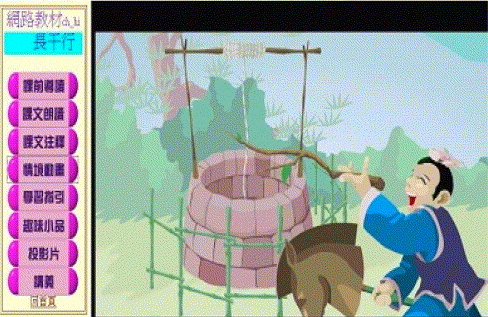
\includegraphics[width=\textwidth]{media1}
 \caption{Poem - High richness media}
    \end{subfigure}\hspace{0.05\textwidth}
    \begin{subfigure}{0.45\textwidth}
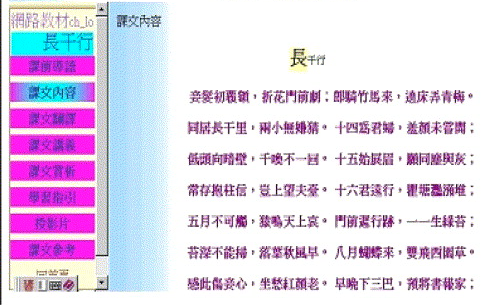
\includegraphics[width=\textwidth]{media2}
  \caption{Poem - Low richness media}
    \end{subfigure}
    \begin{subfigure}{0.45\textwidth}
        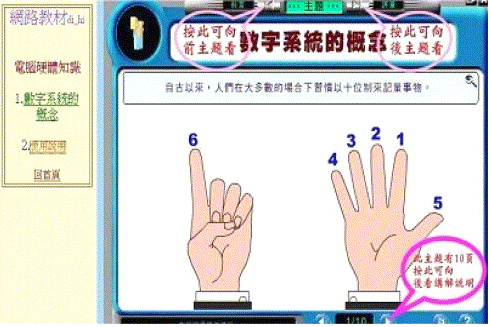
\includegraphics[width=\textwidth]{media3}
        \caption{Number - High richness media }
    \end{subfigure}\hspace{0.05\textwidth}
\begin{subfigure}{0.45\textwidth}
        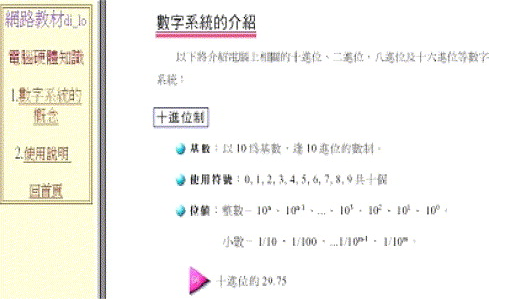
\includegraphics[width=\textwidth]{media4}
        \caption{Number - Low richness media }
    \end{subfigure}
    \caption{E-learning course designs \cite{sun2007design}}
\end{figure}

Sun \& Cheng \cite{sun2007design} evaluated both learning score and learners' satisfaction, they found that for the high uncertainty e-learning curse high media richness provide positive effects on the score and satisfaction. On the other hand, there had no significant different in the score and satisfaction between presenting content with high and low media richness within the low uncertainty e-learning curse. 

Modern education such as e-leaning and m-learning enabled multimedia presentation that could potentially attract learners, too much of the multimedia, however, distract learners. Media Richness Theory had helped defined how much media should be provided an education system. For high ambiguous and uncertain learning content, the rich media such as animation would be appropriate. Meanwhile, for the low ambiguous and uncertain learning content, the rich media was not necessary. 

%%%%%%%%%%%%%%%%%%%%%%%%%%%%%%%%%%%%%%%%%%%%%%%

\subsection{Learning Theory of Andragogy} 

Maturity also had significant effected on how learners learnt. That is to say, adult learners would have different cognitive process and well as be motivated differently to a children learners. 

Cercone (2008) \cite{cercone2008characteristics} predicted characteristics of adult learners that could have implication for the instructional design of online learning. The prediction was mainly grounded on Knwles et al. (1970) \cite{knowles1970modern}'s Learning Theory of Andragogy and was complemented by Lowry (1989) \cite{lowry1989supporting}'s Self-directed Learning , Merriam (1991) \cite{merriamcaffarella}'s Knowledge of Experienced Learning, and Mezirow (1997) \cite{mezirow1997transformative}'s Transformative Learning Theory.  

Cercone (2008) \cite{cercone2008characteristics} proposed thirteen differentiated characteristics of adult learners and provided instructional design recommendations based on the characteristics: 
\begin{enumerate}
\item Adult learners have some limitations - teachers should consider, for example, providing large enough and easy to read fronts, using some visual presentations such as images, charts, and tables, providing a clear structure menu, and ensuring that culture bias was not included within the course
\item They have their individual learning experience and preference, therefore they should be allowed to learn on their own pace - teachers, in addition, should provide enough online learning resources
\item They like to be involved in learning process therefore, they should be allowed to learn autonomously - teachers, in addition, should arrange regular communication sessions to individual and groups
\item They need teachers to provide scaffolding such as coaching audio file, resources, examples, or scenarios to assist them to complete learning tasks
\item They have their own pre-existing learning history and might need sometimes to adjust themselves to learner-centered paradigm - teachers should encourage learner participation and collaboration 
\item They need teachers to be facilitators who arranged appropriate course environment for them and summarized learning lessons for closure. 
\item They have their own prior experience - teachers should include some learning activities that allowed learners to used their prior knowledge, provide clear explanations how new learning topics linked to learners' prior experience
\item They want to see the link how the learning linked to their real lives, therefore teachers should provide learning activities that related to real life situations and encourage learners to apply their own experience to learning
\item They need to feel that learning focused on topics that directly concerned them (i.e., they wanted to know why they should learn things and what benefits they would get from learning that particular subjects) - teachers should provide clear explanations how the learnings would be applied practically
\item They need a self-evaluation to challenge themselves - teachers should reward them for success
\item They prefer collaborative, respectful, mutual - teachers should allowed them to express their opinion and arrange a comfortable learning environment
\item They need a self-reflection - teachers should provide periodic opportunities for learners to discuss how they managed their online course
\item They need dialogue and social interaction - teachers should provide collaboration learning betweens peers 
\end{enumerate}


%%%%%%%%%%%%%%%%%%%%%%%%%%%%%%%%%%%%%%%%%%%%%%%%

\subsection{Activity Theory} 

According to Kuutti (1996)\cite{kuutti1996activity}, Activity Theory (AT) was first developed around 1920s by Lev Semyonovich Vygotsky within Soviet psychology. They defined the AT as "a philosophical and cross-disciplinary framework for studying different forms of human practices as development processes, both individual and social levels interlinked at the same time'' \cite [pp. 23]{kuutti1996activity}. Based on the definition, it was a framework or descriptive theory rather than a predictive theory. AT looked beyond the core of the activity of subjects that interacted with objects to achieve desired outcomes but accounted environment, culture, motivation, mediated tool, and more as elements of an activity system.

 Engestr{\"o}m (1987) \cite{engestrom1999perspectives} presented the activity triangle model (Figure 2.x) that helped explain how these wide range of elements worked together. The subjects were socio-culturally embedded actors that interacted with objects within the community through the use of instruments, rules, and division of labour.

\begin{figure}[!hbt]
\centering
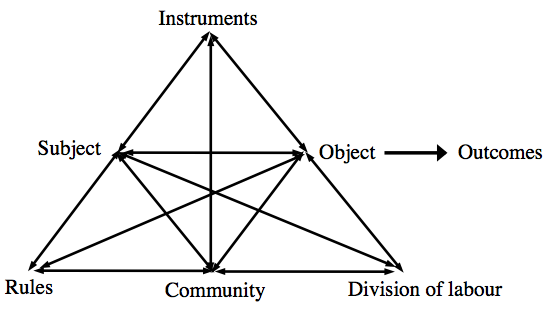
\includegraphics[width=0.7 \textwidth]{ac2}
\caption{Example of a personal-mobile knowledge and learning organization system \cite{vavoula2002kleos}}
\end{figure}

\subsubsection{Cultural-Historical Activity Theory} 

Cultural-Historical Activity Theory (CHAT) had three significant compositions: cultural theory, historical theory, and activity theory. According to Foot (2014) \cite{foot2014cultural} "Cultural points to the premise that humans are enculturated, and everything people do is shaped by and draws upon their cultural values and resources" \cite[pp. 3]{foot2014cultural} and since the cultures were gradually developed over time, to analyzed peoples' behavior, the historical path of the behavior should also be also considered. CHAT, same with the Activity Theory (AT) presented in section 2.x, was also a framework or descriptive theory that explained and provided understanding of human activity. However, CHAT included not only the interrelationship between the six elements presented in Engestr{\"o}m (1987) \cite{engestrom1999perspectives}' s the activity triangle model (Figure 2.x) but also cultural and historical dimensions. 

For teaching and learning activity, AT could contribute to a better understanding of how an instrument mediated learning activity and be used a framework to evaluate its applicability within a particular learning context. For example, Waycott et al. (2005) \cite{waycott2005pdas} adopted AT to analze applicability of PDAs (i.e., as an instrument) to support a life long learning within three particular learning contexts: distance learners used e-book on PDAs; industrial workers used PDAs to access to information when they were away from their offices; and using PDAs in an art gallery. The first two contexts were similar in the way that the learners owned the PDAs and they used it stationary when they were sitting at a desk or in a train. Meanwhile in the third context, PDAs were loaned to the learners and they used it when they were roaming around the art gallery.

Observation results indicated that the learners that were the subject of the system integrated their past experiences, personal preference, motivation, and daily schedule into their PDAs adoption. They reported that PDA could support life long learning, however, some of PDAs novice faced difficulties typing on PDAs and preferred to use a computer keyboard. However, the PDAs that were the instrument of the learning system could not completely replace other tool such as laptops and desktop computers because PDAs could not support every required activity. For example, it did not allow the learners to take personal notes when they were roaming around the art gallery. Thus, the role of the PDAs was a complimented instrument within these particular learning contexts.


%%%%%%%%%%%%%%%%%%%%%%%%%%%%%%%%%%%%%%%%%%%%%%




%%%%%%%%%%%%%%%%%%%%%%%%%%%%%%%%%%%%%%%%%%%
%%%%%%%%%%%%%%%%%%%%%%%%%%%%%%%%%%%%%%%%%%%

\section{Interface Design Guidelines}

The Transactional Distance Theory (TDT) contributed functional design guidelines of m-learning. However, the TDT-theoretical guidelines lacked of guiding towards interface design that was another important aspect to make the design usable, easy, and pleasant to learners. Unfortunately, according to Dix (2009) \cite{dix2009human}, designing the usability for a new application such as m-learning took a lot of time and required many skills. Dix (2009) \cite{dix2009human} further suggested developers to take a shortcut by following exiting best practices which commonly were encapsulated inform of usability design guidelines, design principles, or heuristics. There were three long-standing design guidelines for global interactive system that influenced many following interface design guidelines for general mobile devices and modern education platform such as e-learning and m-learning. 

\subsection{Basic Design Check lists} 
Firstly, in 1988, Norman \cite{norman1988psychology} proposed four basic design check lists that highlighted the important of users and aimed to provide ease-of-use. The check lists were: 
\begin{enumerate} 
\item Provide visibility - make all available options to be easily visible to users 
\item Provide feedbacks - give clear explanations on the consequence of user's action 
\item Provide good conceptual model - make the overall design of the system easy for users to draw a conceptual map how system work together thus they could link relationships between different parts and navigate themselves though the system
\item Provide clear mapping between goals and required actions, the action and results, and the results and achievements
\end{enumerate} 

Figure 2.x presents example of an m-learning application evaluation based on Norman (1988) \cite{norman1988psychology}'s check lists. The application was called "iLearn Geography", downloaded from Apple's app store on September \nth{5}, 2017. 

\begin{figure}[!hbt]\centering
    \begin{subfigure}{0.25\textwidth}

\includegraphics[width=\textwidth]{design1}
\caption{Main menu}
    \end{subfigure}\hspace{0.05\textwidth}
 \begin{subfigure}{0.25\textwidth}
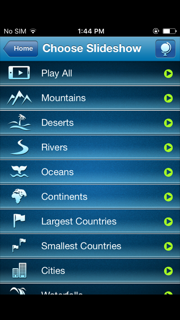
\includegraphics[width=\textwidth]{design4}
\caption{Sub-menu}
 \end{subfigure}\hspace{0.05\textwidth}
 \begin{subfigure}{0.25\textwidth}
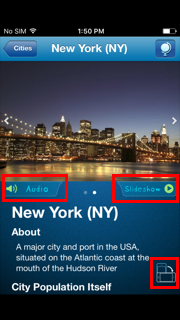
\includegraphics[width=\textwidth]{design3}
\caption{Text content}
    \end{subfigure}\hspace{0.1\textwidth}
 \begin{subfigure}{0.55\textwidth}
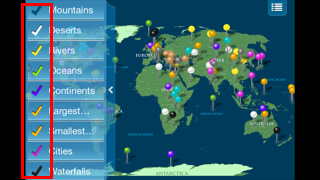
\includegraphics[width=\textwidth]{design2}
\caption{Graphical content }
    \end{subfigure}\hspace{0.1\textwidth}
  \caption{Screen shots of "iLearn Geography" a m-learning application downloaded from Apple's app store}
\end{figure}

Based on the check list \cite{norman1988psychology}, overall, the application provide high visibility as it adopted menu interface design to show available options (Figure 2.xa and 2.xb) as well as presented icons that inform actions. For example using a speaker icon to inform learners that they could possible listen to some audio files and use screen rotation icon to inform that they could rotate the screen (Figure 2.xc, as marked in red squares). It also provided a good conceptual model as it presented hierarchical menu (Figure 2.xa and 2.xb) that helped the learner to draw overall concept of the application and aided them to navigate trough the application smoothly. Additionally, it provided pretty clear mapping between intentions, required action, results, and achievement as it provided some clear options on the menus, the learners could tap on the provided menus resulting in opening their preference view either list view, map view or slides show. On the other hand, the application provided a double-edged feedback. Even though, it provided clear menu titles as well as used colour differentiation and tick sign to lead learners that there were some required actions (Figure 2.xd, as marked in red square), it did not provide any clear instruction that how to interact with the map. Without the clear instruction, the learners might missed some important learning content. 

\subsection{Eight Golden Rules of Interface Design} 

Secondly, Shneiderman (1988) \cite{shneiderman2010designing}, proposed "Eight Golden Rules of Interface Design". Similar to the Norman \cite{norman1988psychology}'s guidelines, it had user-centered concept, ensured interface design effectiveness, and usability. The eight golden rules were: 

\begin{enumerate} 
\item Strive for consistency - provide language consistency and make sure, in similar situations, users sre required to act in consistent sequences
\item Enable frequency users to use short cuts - reduce operations for any regular performance 
\item Offer informative feedback 
\item Design dialogue to yield closure - inform users clearly where they are, what they are doing, and provide them with closure when they accomplish any task
\item Offer simple error handling - provide a design in which users can not make a serious error, if they make one, provide them provide them a simple and comprehensible solution
\item Permit easy reversal of actions - if users make any input mistake, allow them to undo their action
\item Support internal locus of control - allow users to feel in control of the system and they are the one who initiate some actions
\item Reduce short-term memory load - do not burden users with any complicated sequence, code, number, or other information that are processed with their short-term memory 
\end{enumerate} 

The eight golden rules of interface design influenced many later interface design guidelines for mobile devices. When the guidelines were narrowed down to to concentrated more on the specific devices, it included some design techniques with regards to the small displays and mobility. 

For example, grounding on Shneiderman (1997) \cite{shneiderman2010designing}'s eight golden rules of interface design, Gong \& Tarasewich (2004) \cite{gong2004guidelines} proposed guidelines for interface design of hand-held mobile devices in which four rules were reminded unchanged (i.e., enable frequency users to use shortcuts, offer informative feedback, design dialogue to yield closure, and support internal locus of control), four rules were modified: 
\begin{enumerate} 
\item Consistency - besides the language consistency, as mobile devices have many operating system, provide media display consistency (e.g., text, audio, and visual presentation) across these platforms 
\item Reversal of actions – a mobile devices had less memory storage to store the past events
\item Error prevention and simple error handling – as small buttons of mobile devices increased potentials of mistaken action, users should not be allowed to perform a simple action (e.g., one press power on/off) that had harmful consequences (e.g., lose all stored-data)
\item Reduce short-term memory load – as mobile devices users had more possibility to get distract by surroundings (e.g., when they used the device on their move), thus provided alternative interactions such as using voice control instead of button press to activate some features
\end{enumerate} 

and seven guidelines were added: 

\begin{enumerate} 
\item Design for multiple and dynamic context - allow users to adjust display output such as brightness and volume to suit immediate context
\item Design fro small devices - provide alternative interactions for example speech input could be used alternatively with small virtual buttons and audio output might might be used alternatively with text and graphics
\item Design for limited and split attention – provide interface designs that require as little attention as possible, for example, audio or tactile output could be used rather than visual displays
\item Design for speed and recovery – as mobile devices users would easily lose their interest if they needed to wait for a few seconds, provide a quick access and a secure save function
\item Design for top-down interaction – present information through hierarchical mechanism
\item Allow personalisation – as mobile devices were more personal compared to other stationary computers, allow some self configurations
\item Design for enjoyment – mobile interface design should be useful, fun, and visually pleasing
\end{enumerate} 

Jones \& Marsden (2006) \cite{jones2006mobile}also presented some guidelines that grounded on the eight golden rules with regards to the mobile devices' hardware constraints. They suggested using menu interface design and arranging it either in either concave or wide-shallow tree hierarchical order, using icon in the menu title to provide visual entertaining, providing on-screen manual if the screen of target's device were big enough and otherwise opting for online manual, and provided summarized and concise content with bolding or tilting to help users in skim reading. 

Thirdly, Nielsen \& Molish (1990) \cite{nielsen1990heuristic} proposed heuristic evaluation as an inspection method for investing software usability in general. 

%%%%%%%%%%%%%%%%%%%%%%%%%%%%%%%%%%%%%%%%%%%


\subsection{Heuristic Design Guidelines}

In 1990, Nielsen \& Molich (1990) \cite{nielsen1990heuristic} tried to reduced the complexity of investigation of software usability by specifying nine usability heuristics as a check list for user interface evaluation including: simple and natural dialogue; speak the user's language; minimize user memory load; be consistent; provide feedback; provide clearly marked exits; provide shortcuts; good error messages; and prevent errors. 

They further suggested that the heuristic evaluation could be done at the early stage of the development process by a small group between three to five evaluators who were independent from each other. The evaluators would inspect and judge an interface design according to the heuristic list and report positive and negative aspects of the interface. Therefore, this evaluation technique was cost effective and required minimal advance planning. 

Later on, Nielsen (1995) \cite{nielsen199510} published an improved list included ten concrete usability heuristic evaluation criterion: 
\begin{enumerate}
\item Visibility of system status - inform users what is going on with appropriate feedback within reasonable time
\item Match between system and the real world – use language that users are familiar not the system-oriented terms and present them logical order 
\item User control and freedom - provide "undo" and "redo" options for users so they could exit or retrieve their actions 
\item Consistency and standards - follow platform convention and make sure all words and actions are consistent throughout the system 
\item Error prevention - provide a clear indication to avoid error. If there is one, provide a clear error message 
\item Recognition rather than recall - make all objects, actions, and options visible to users. They should not need to remember any information or instruction from screen to screen. 
\item Flexibility and efficiency of use - design for both experienced and inexperienced users by allowed user's configuration to suite their competency and preference 
\item Aesthetic and minimalist design - only present relevant dialogue 
\item Help users recognize, diagnose, and recover from errors - inform users about errors in understandable language and provide them with constructive solution
\item Help and documentation - provide help and documentation that were easy to be found by users, clearly list what they should do in concrete steps
\end{enumerate} 

Much research extended Nielsen (1995) \cite{nielsen199510}'s heuristic check list to evaluate some specific domains. For example, Reeves et al. (2002) \cite{reeves2002usability} adopted some of Nielsen \& Molich (1990) \cite{nielsen199510}'s original heuristic work, applied them into e-learning context , and added more heuristic evaluation check lists to cover all aspects of e-learning. The following list presents Reeves et al. (2002)'s extended check lists and examples of questions that evaluators could ask themselves when they evaluated an e-learning system \cite[pp.4-6]{reeves2002usability}.

\begin{enumerate}
\item Navigation support 
\begin{itemize}
\item Does the interface of the e-learning program speak for itself so that extensive consultation of a manual or other documentation does not interfere with learning? 
\item Does the e-learning program provide user-friendly hints and/or clear directions when the learner requests assistance? 
\item Does the e-learning program include a map or table of contents that allows the learner to see what has been seen and not seen? 
\end{itemize}
\item Interactivity
\begin{itemize}
\item Does the e-learning program provide meaningful interactions for the user, rather than simply presenting long sections of text? 
\item Does the e-learning program engage the learner in content-specific tasks to complete and problems to solve that take advantage of the state-of-the-art of e-learning capabilities?
\end{itemize}
\item Message design 
\begin{itemize} 
\item Is the most important information on the screen placed in the areas most likely to attract attention?
\item Does the e-learning program follow good information presentation guidelines for organization and layout?
\end{itemize}
\item Learning design 
\begin{itemize}
\item Does the e-learning program follow an appropriate learning design to achieve its stated objectives?
\item Does the e-learning program engage learners in tasks that are closely aligned with the learning goals and objectives?
\end{itemize} 
\item Media integration
\begin{itemize}
\item Is media included that is obviously superfluous, i.e., lacking a strong connection to the objectives and design of the program?
\item Is the most appropriate media selected to match message design guidelines or to support instructional design principles?
\item If appropriate to the content, are various forms media included for re-mediation and/or enrichment?
\end{itemize}
\item Instructional Assessment  
\begin{itemize}
\item If appropriate to the content, does the e-learning program provide opportunities for self-assessments that advance learner achievement?
\item If appropriate to the content, do assessments provide sufficient feedback to the learner to provide remedial directions?
\item Wherever appropriate, are higher order assessments (e.g., analysis, synthesis, and evaluation) provided rather than lower order assessments (e.g., recall and recognition)?
\end{itemize}
\item Resources
\begin{itemize}
\item Does the e-learning program provide access to a range of resources (e.g., examples or real data archives) appropriate to the learning context?
\item If the e-learning program includes links to external World Wide Web or Intranet resources, are the links kept up-to-date?
\item Are resources provided in a manner that replicates as closely as possible their availability and use in the real world?
\end{itemize} 
\item Feedback
\begin{itemize}
\item Is the feedback given at any specific time tailored to the content being studied, problem being solved, or task being completed by the learner?
\item Does feedback provide the learner with information concerning his/her current level of achievement within the program?
\item Does the e-learning program provide learners with opportunities to access extended feedback from instructors, experts, peers, or others through e-mail or other Internet communications?
\end{itemize}
\end{enumerate} 

Yanez et al. (2004) \cite{yanez2014heuristic} also applied the same methods when building their heuristic evaluation check lists for mobile devices. Most of their check lists  were grounded on Nielsen \& Molich (1990) \cite{nielsen199510}'s original heuristic work. They adjusted them into mobile devices context and added some new check lists from mobile device interface design best practice and recommendations. The following list presents Yanez et al. (2004)'s additional check lists and its examples questions that evaluators could asked themselves when they evaluated a mobile device's design \cite[pp. 10]{yanez2014heuristic}.
\begin{enumerate}
\item Skills 
\begin{itemize}
\item If the system supports both novice and expert users, are multiple levels of error massage detail available? 
\item Do the selected input device(s) match user capability?
\end{itemize}
\item Pleasure and respectful interaction 
\begin{itemize}
\item Protect users' work, also as for data entry screens with many fields or in which source documents may be incomplete, can users save a partially filled screen?
\item Are typing requirements minimal for question and answer interface?
\end{itemize}
\item Privacy
\begin{itemize}
\item Can protected areas completely inaccessible?
\item Can protected or confidential areas be accessed with certain passwords?
\end{itemize}
\end{enumerate} 

Besides these three well-known design guidelines, O'Malley et al. (2003) \cite{o2003guidelines} presented of an m-learning interface design best practice collection. The collection 

%%%%%%%%%%%%%%%%%%%%%%%%%%%%%%%%%%%%%%%%%%%%
%%%%%%%%%%%%%%%%%%%%%%%%%%%%%%%%%%%%%%%%%%%%
\subsection{M-learning Interface Design Best Practices} 

O'Malley et al. (2003) \cite{o2003guidelines} presented a total of twenty-seven categories of m-learning design best practices that were collected from m-learning case studies and past literatures. The collection included many guidelines aspects for example the guidelines how to adopt PDA for collaboration learning, the guidelines how to provide training to teachers, the guidelines how to choose appropriate mobile technologies in specific learning context, and usability guidelines that assured system assistance. According to O'Malley et al. (2003) \cite{o2003guidelines}, these guidelines could be used by system designers, usability engineers, or teachers. This section only presents some of the guidelines that guided the interface design of m-learning which O'Malley et al. (2003) \cite{o2003guidelines} collected from Alessi \& Trollip (2000) \cite{alessi2000multimedia}'s how to apply multimedia in learning. 
\begin{enumerate} 
\item General learner control 
\begin{itemize} 
\item Do not use timed pause
\item Allow learners to navigate back to review the previous screens
\item Use consistent global interface design
\item Provide control functions such as pause, play, and stop for audio and video media
\item Provide alternatives learners who might have varied learning skills
\item Allow learner control in problem solving tasks
\item Use system control when mastery of content had critical consequences
\end{itemize} 
\item Input 
\begin{itemize}
\item Button - limit number of button in one screen, if the screen requires a large control, consider using menu instead; provide clear feedback (e.g., color change); provide interaction (e.g., cursor change) when conveying functions
\item Menu - use progress menu to advice learners where they are in the application; in hierarchical menu, provide only a few level; if the menu navigation is complex, consider using flow chart of diagram instead; provide simple and clear menu title; provide "exit" or "return" options
\item Hyperlink - for global controls, avoid using hyperlink and use menu instead; for frequent controls, use button instead; keep hyperlink title clear and understandable to learners; provide interactions (e.g., cursor changes and rollovers) to inform learners' action
\end{itemize} 
\item Output 
\begin{itemize} 
\item Text - make sure highlighted text will not be confused with hyperlink; consider using paging technique over scrolling to avoid problem when the text is displayed in vary rang of display; indicate clearly when learners moves to the next section (e.g. provide "click here for next section: section title")
\item Graphics and Animation - they may steal learners' attentions from text content, thus use them only when they benefits learning; they should be consisted with other media in an application; allow control functions (e.g. pause, play, and stop) in animation; pictures should not automatically disappear without any learners' input 
\item Video - same with the graphics and animation, reserve using video only if it benefits learning; generally a video should not be longer than 20-30 seconds; provide learners controls (e.g. pause play, and stop)
\item Sound - consider using audio to get attention and direct learners specially when learners are paying attention on surroundings (e.g., when learners are roaming around museum)
\end{itemize} 
\item Questioning 
\begin{itemize} 
\item Multiple choices - provide at less three alternatives to eliminate likelihood of guessing; the alternatives must be plausible and should not provide any hint to the correct answer
\item Completion or Cloze - only significant words should be blanked out; the position of the blank should be near the end of the statement; and one statement should not contain many blanks to maintain its original meaning
\end{itemize} 
\end{enumerate} 
















%%%%%%%%%%%%%%%%%%%%%%%%%%%%%%%%%%%%%%%%%%%
%%%%%%%%%%%%%%%%%%%%%%%%%%%%%%%%%%%%%%%%%%%
\newpage
\section{Learner Persona}

Although, grounding functionality design and interface design of mobile learning (m-learning) application on Transaction Distance Theory (TDT) and existing best practices would possible ensure leaning quality and usability, as the design would be used by specific group of learners, the design process still required a user study. 


 In menu-based voice interface for telephone system, if developers did not consider limitations of human working memory which was small and rapidly blown away, they might overload users' memory with too many choices (e.g., press 1 to ..., press 2 to ..., press 3 to ..., and so on), the users might forget these choices and made a mistake. Therefore, according to Jones \& Marsden (2006) \cite{jones2006mobile} understanding user was an important activity in mobile interaction design process and some basic knowledge about human cognitive process would help developers to choose a better design choice. Parsons et al. (2006) \cite{parsons2006study} added that identifying m-learning users would help developers to target a better personalised learning. 

To understand users, developers needed to conduct a user study. There were many available techniques such as, suggested by Jones \& Marsden (2006) \cite{jones2006mobile}, field studies and direct questioning

\begin{itemize} 
\item The field studies - developers could observed how users interacted with other users and environment in a real situation for an extended period of time
\item The direct questioning - developers could take control of the observation and be more specific by asking users some directed questions in an interview session of a focus group. This technique was mostly used to validate the developers' interpretations and gain additional information from the field study. 
\end{itemize}

According to Jones \& Marsden (2006) \cite{jones2006mobile}, those information from the user study had to be transcribed, organized and presented in an proper form in order to capture some key elements and design issues that directed the development team and informed a usable and effective design. However, Pruitt \& Adlin (2010) \cite{pruitt2010persona} claimed that these were challenge tasks. A development team might find it was hard to identify which piece from a huge collection of users' information was useful for the design, after correctly identifying the useful information, each developer in the team might interpret the information in different ways, after everyone in the team shared the same understanding about the users, how the understand could direct their design decision, and after they made the decision, how the understanding be used to ensure design effectiveness. 


According to Dix (2009), in Human Computer Interaction (HCI), the knowledge about the users could be presented in many ways. For example, persona that was a descriptive fiction that represented real users; scenario that was a story that informed how a design was used; hierarchical task analysis that arranged users' performance hierarchically to provide understanding how users managed to achieve their goals; and dialogue specification that focused interaction of users' input and system's response.

\subsection{Persona} 

The persona was first introduced in 1999 by Alan Cooper \cite{copper1999inmates} to explained customers' behavior in marketing researches. Cooper (1999) \cite{copper1999inmates} defined the persona as \textit{a character} that was created by gathering behavioral data from real users. Later on, much researchers used different word to define persona. For example, Pruitt \& Adlin (2010) \cite{pruitt2010persona} defined it as \textit{a fiction character}, meanwhile Idoughi et al (2012) \cite{idoughi2012adding} defined it as \textit{a descriptive model of user} and further explained that the persona contained some of the user' information such as his/her characteristics, goals, and needs.

Pruitt \& Adlin (2010) \cite{pruitt2010persona} claimed that the persona was different form other HCI presentation techniques because "Persona offered a consistence target-audience vision" \cite[pp.18]{pruitt2010persona}. It was fun, informal characters that can better inspire imagination for the design team, help captivate them and provide them with memorable information to be incorporated into the design process. 

In addition, according to Pruitt \& Adlin (2010) \cite{pruitt2010persona} persona had some benefits:

\begin{itemize}
\item When a design team had many conflicting hypotheses about their users, the use of persona could help clarify and refine these hypotheses, thus enabling the design team to work in harmony and make concrete design decisions
\item It was not limited to identifying the majority user groups, it could also be used to recognize other minority groups, expanding the design to represent everyone within the user group spectrum
\item At the beginning of the development process, it was common to have many proposed ideas on the design. With limited resources, it might be paramount for the design team to focus on designs that were possible and worth developing. Persona could assist them in creating focused designs that met the needs of the target audience while making the most out of limited resources
\end{itemize}

Much research created and used personas in their user studies. For example, Rahim et al. (2014) \cite{rahim2014engineering} created personas representing users' background and their behavior when they purchased food products, with the aims to explore users' requirement, and contribute to their Halal-Checker Mobile Application (I-scan) design. 

Calvo et al. (2014) \cite{calvo2014user} also created personas characterising a group of students and teachers with disabilities. The personas were used to improve the performance of synchronous chatting within an m-learning application. 


\subsection{Scenario} 

According to Jones \& Marsden (2006) \cite{jones2006mobile}, scenario had the same propose as the persona, to present detail of users' character, it, however, focused on the actions that these users carried out. 

Including a learners study into the design process contributed to a usable and effective m-learning design that suited a specific group of learners. Persona could represent these learners and describe their learning goals, attitude, and behavior. The persona could be shared among people involved in design process, direct their design decisions, and ensure the design's usability and effectiveness. 


%%%%%%%%%%%%%%%%%%%%%%%%%%%%%%%%%%%%%%%%%%%
%%%%%%%%%%%%%%%%%%%%%%%%%%%%%%%%%%%%%%%%%%%
\newpage 
\section{Mobile Learning Application Design}

According to Dix (2009) \cite{dix2009human}, although grounding design on best practices could ensure usability, design a quality interface still required an iterative process. Dix (2009) \cite{dix2009human} further suggested prototyping technique which allowed users to experience a prototype and then the users and/or developers would evaluate its usability. Depending on the evaluation results, the prototype might need a redesign. This process would loop until usability reached an acceptable level. 

%%%%%%%%%%%%%%%%%%%%%%%%%%%%%%%%%%%%%%%%%%%
%%%%%%%%%%%%%%%%%%%%%%%%%%%%%%%%%%%%%%%%%%%

\section{Mobile Learning Application Evaluation}

Dix (2009) \cite{dix2009human} introduced two types of usability evaluation method: laboratory experiment method which users would perform tasks under some controlled conditions in a laboratory setting and field study method which users would perform tasks in an actual environment. 



%%%%%%%%%%%%%%%%%%%%%%%%%%%%%%%%%%%%%%%%%%%
%%%%%%%%%%%%%%%%%%%%%%%%%%%%%%%%%%%%%%%%%%%










